% So we make this "beamer" rather than document! 

\documentclass{beamer}
\usetheme{default}
\usecolortheme{beaver}
\setbeamertemplate{navigation symbols}{}

\usepackage{beamerfoils}
%\usepackage{natbib} 
\usepackage[natbib=true, bibstyle=authoryear, citestyle=authoryear-comp]{biblatex}
\usepackage{graphicx} 
%\usepackage{geometry}
\bibliography{/Users/Nick/Dropbox/Dropbox_Documents/my_library}
%\bibliographystyle{apalike}


%\setbeameroption{show notes}
%\setbeamertemplate{note page}[plain]

\title{Understanding Rural Private School Performance}
\author{Nick Eubank}
\date{\today}


% This is the beginning of a real document!
\begin{document} 

\begin{frame}{}
	\titlepage
\end{frame}

\begin{frame}{Context}
	\begin{enumerate}
		\item \textbf{Massive growth in rural private enrollment. }
			\begin{itemize}
				\item \cite{Andrabi:2008ji, Pratham:2005vw}
			\end{itemize}
		\pause
		\item \textbf{Private schools outperform government schools.}
			\begin{itemize}
				\item \cite{Jimenez:1991wa, Jimenez:1995vg, Pratham:2005vw, Andrabi:2011hl, Desai:2009ty, Tooley:2003vf, Alderman:2003we, Alderman:2001wk}
		\end{itemize}	
		\pause
		\item \textbf{Big push for voucher programs.}
		\begin{itemize}
			\item \cite{Chakrabarti:2008vc, Kelkar:2006tq, Panagariya:2008wi}
		\end{itemize}
	\end{enumerate}
\pause
But \emph{why} are private schools better?
\note{Enrollment in Pak increased by 47\% from 2000 to 2005. In 2005, was 1/3. In India, greater than 20\%.}

\end{frame}


\begin{frame}{Explanation 1: Teaching Quality}

Possibility 1: Better Inputs
\begin{itemize}
	\pause
	\item No
\end{itemize} 
\pause	

Possibility 2: Better Induced Effort
	\begin{itemize}
		\item Pay for performance, fire bad teachers.
		\pause
		\item Clearly improvement over public schools. 
		\begin{itemize}
			\item \cite{Muralidharan:2008tb, Chaudhury:2006vp}
		\end{itemize}
		\pause
		\item Importance shown in US research.
		\begin{itemize}
			\item \cite{Hanushek:1997tt,Hanushek:2003hz,Banerjee:2007wx}
		\end{itemize}
	\end{itemize}
\end{frame}


\begin{frame}{Explanation 2: Sorting}
Maybe private school students are ``different.''
\pause
	\begin{itemize}
			\item $>$20\%  send one child to a private school and one child to a government school.
			\pause
		\item Some attempts to control through randomization of vouchers
			\begin{itemize}
				\item \cite{Angrist:2002up, Bellei:2008uu}
			\end{itemize}
		\pause
		\item But lots of problems...
			\begin{itemize}
				\item Risk of losing vouchers induces efforts
				\item Selective admission
			\end{itemize}
	\end{itemize}	

\pause
If true, then private school superiority is illusory. 
\begin{itemize}
	\item Vouchers could result in massive mis-allocation of resources.
\end{itemize}
\end{frame}


\begin{frame}{This Paper}
\pause	
Private school dominance declines by 50\% in fractionalized villages
	\pause
\begin{enumerate}
	\item This does \emph{not} arise because of changes in ``Teaching Quality''
	\item This \emph{does} arise because of changes in ``Sorting.''
	\pause
		\begin{itemize}
			\item In homogeneous villages, school choice is based on academic potential.
			\pause
			\item In fractionalized villages, school choice is based on caste politics.
		\end{itemize}
\end{enumerate}
\pause
Tells us that \emph{at least} half of private school premium comes from selective sorting, not better teaching.
\end{frame}



\section{Methodology}\label{}
\begin{frame}{Outline}
	\tableofcontents[currentsection]
\end{frame}

\begin{frame}{Data}	
Learning and Educational Attainment in Punjab Schools (LEAPS)
\begin{itemize}
	\item 2003-2007 panel data with data from teachers, students, households, and owners.
	\item One four year panel (12,110 children)
	\item One two year panel (11,852 children)
	\item Includes: Child Test Scores, Teacher Test Scores, Parental Educational, HH Wealth
	\item Test scores are normalized using IRT -- mean 0, standard deviation 1.
	\item 112 Villages in Three Districts
\end{itemize}
\end{frame}

\begin{frame}{}
	\begin{figure}[htb]
		\begin{center}
		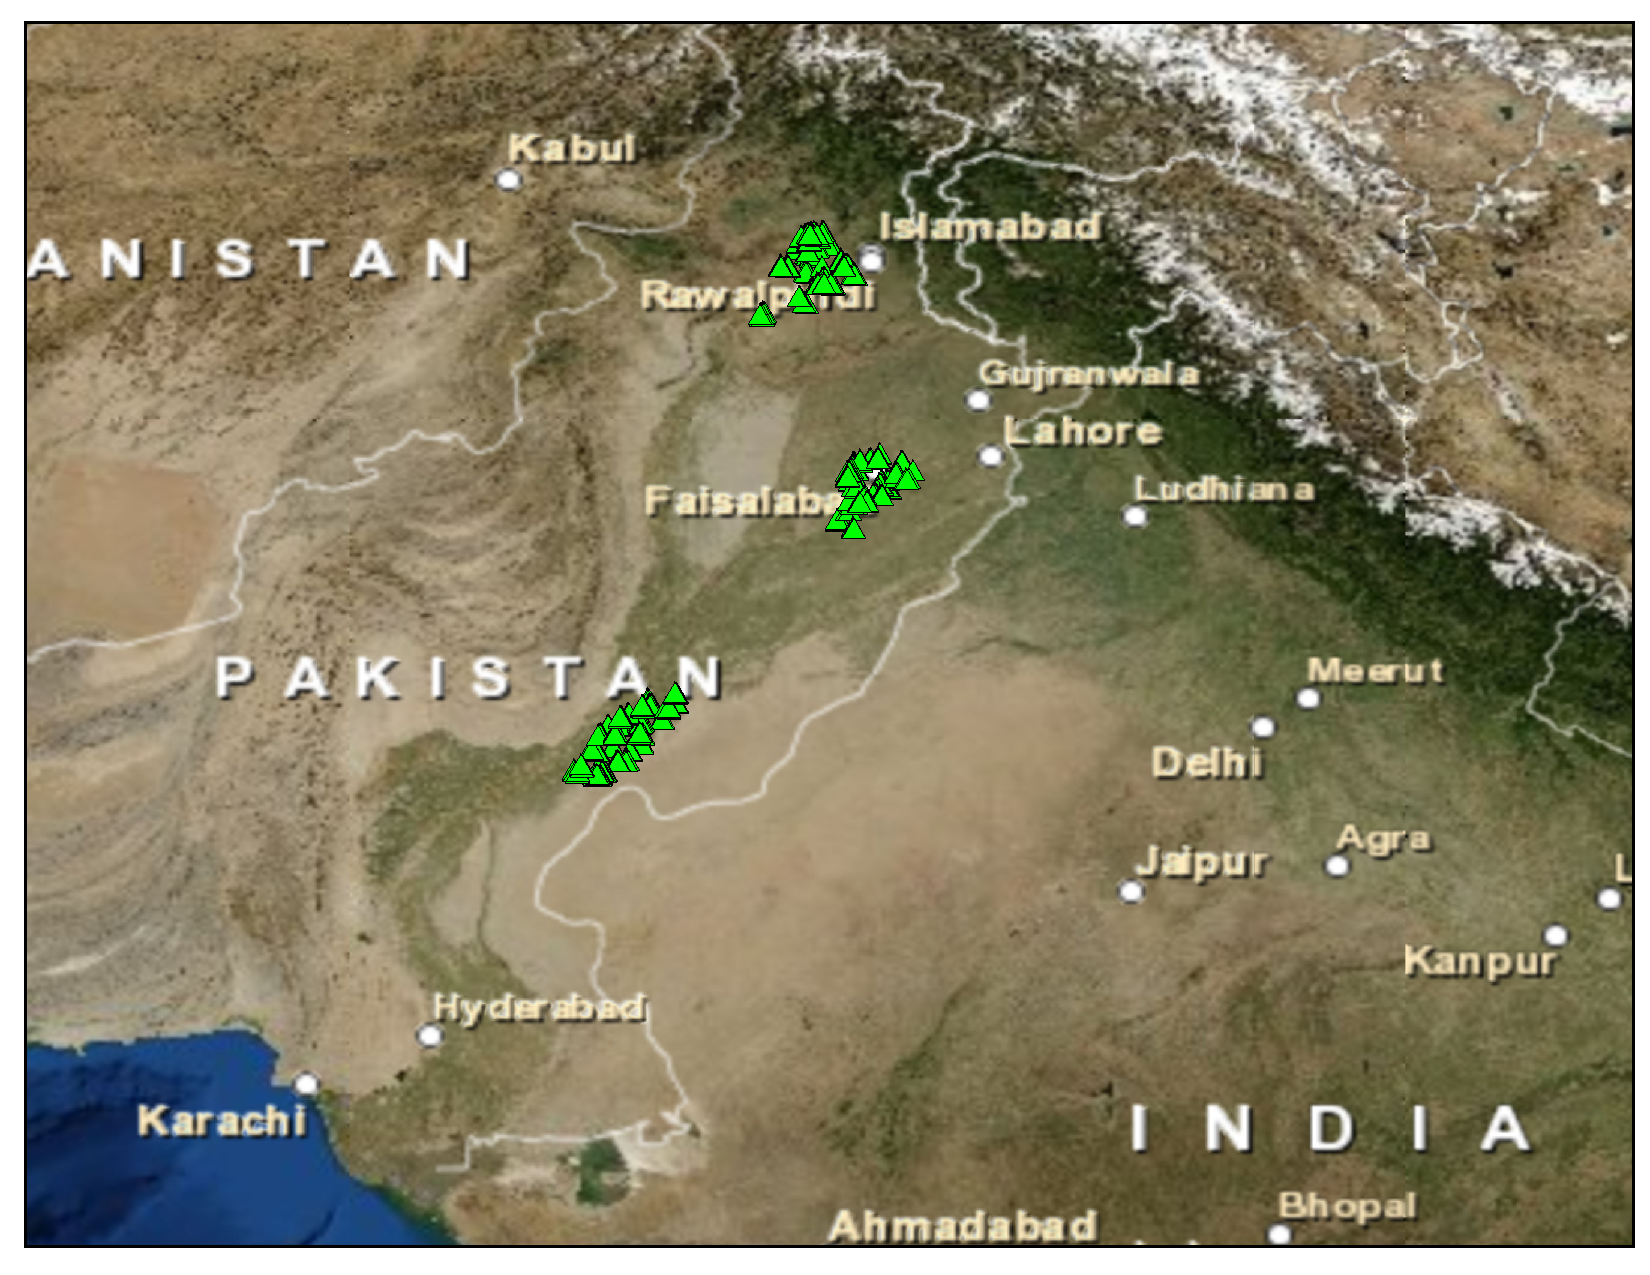
\includegraphics[scale=0.4]{maps/hh_map_allpak.pdf}
		\end{center}
	\end{figure}
\end{frame}


\begin{frame}{}
	\begin{figure}[htb]
		\begin{center}
		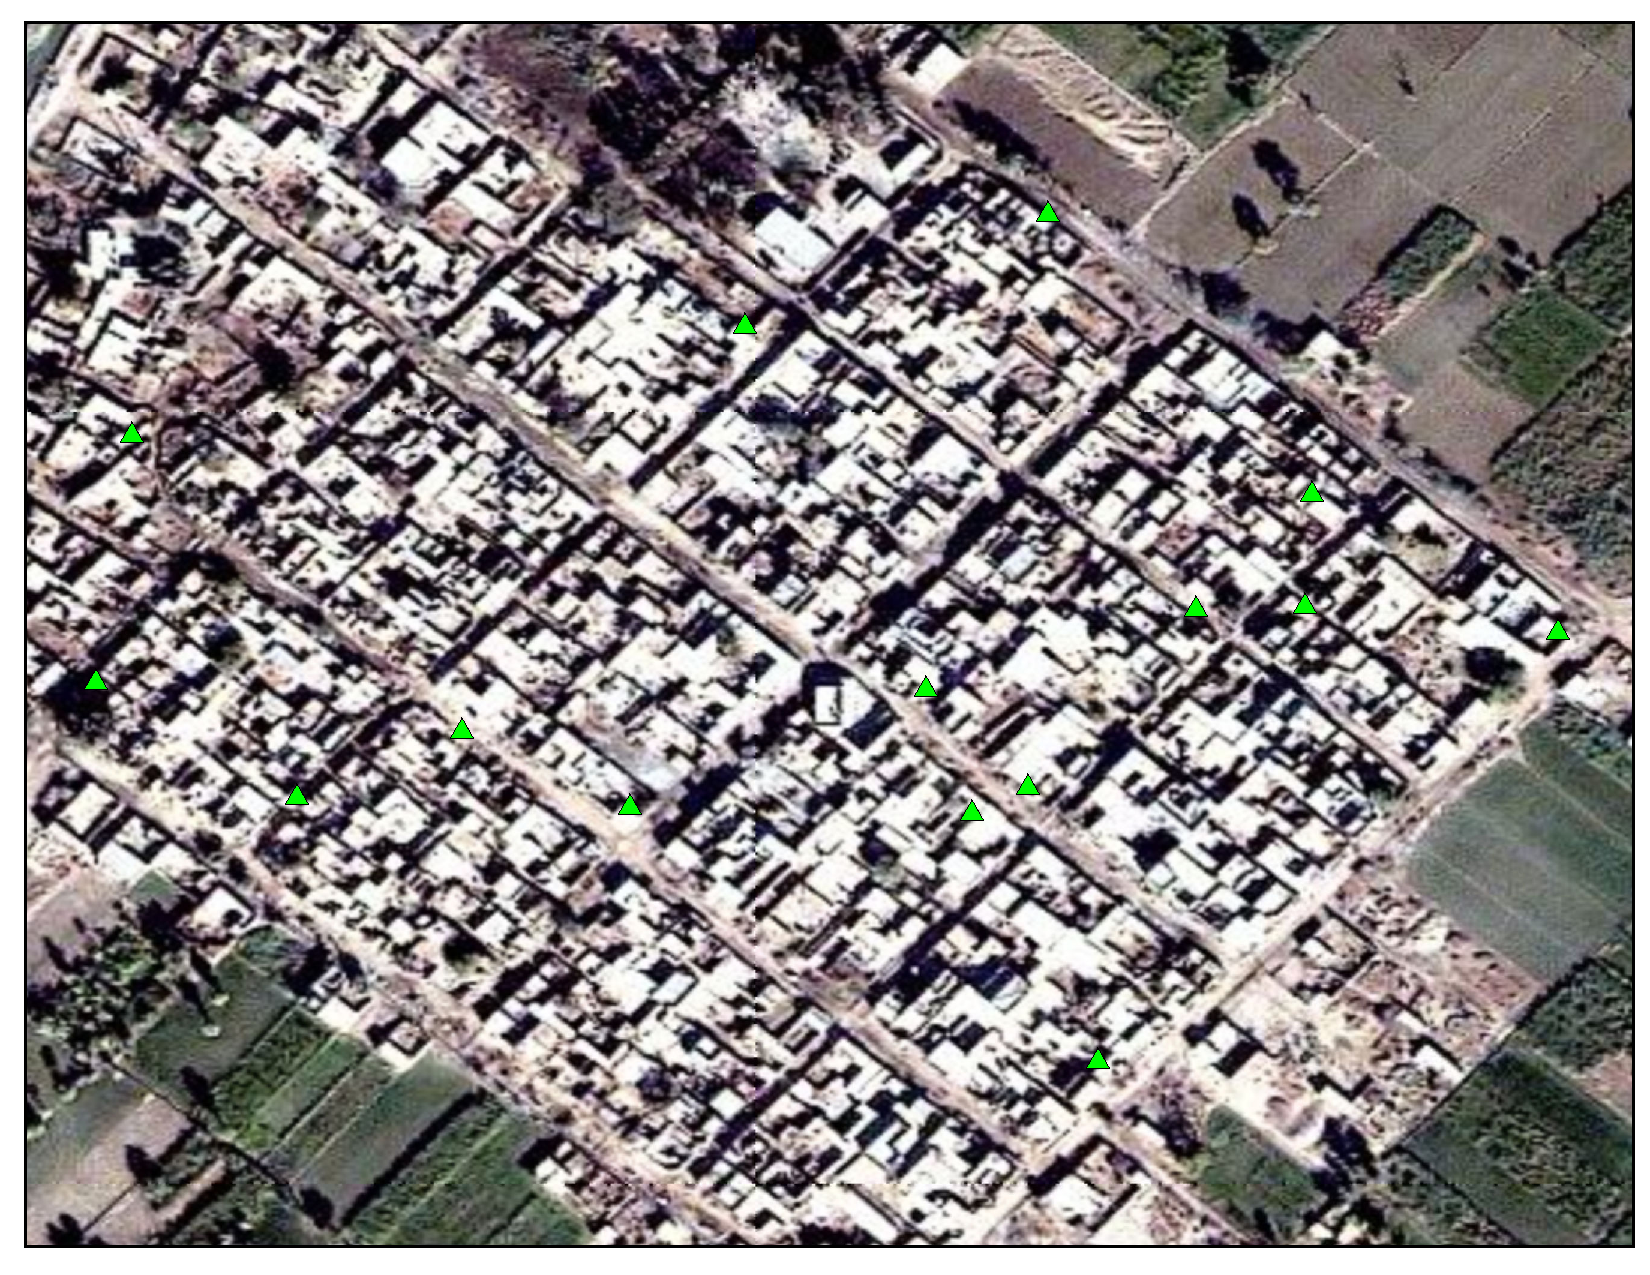
\includegraphics[scale=0.4]{maps/concentrated.pdf}
		\end{center}
	\end{figure}
\end{frame}

\begin{frame}{}
	\begin{figure}[htb]
		\begin{center}
		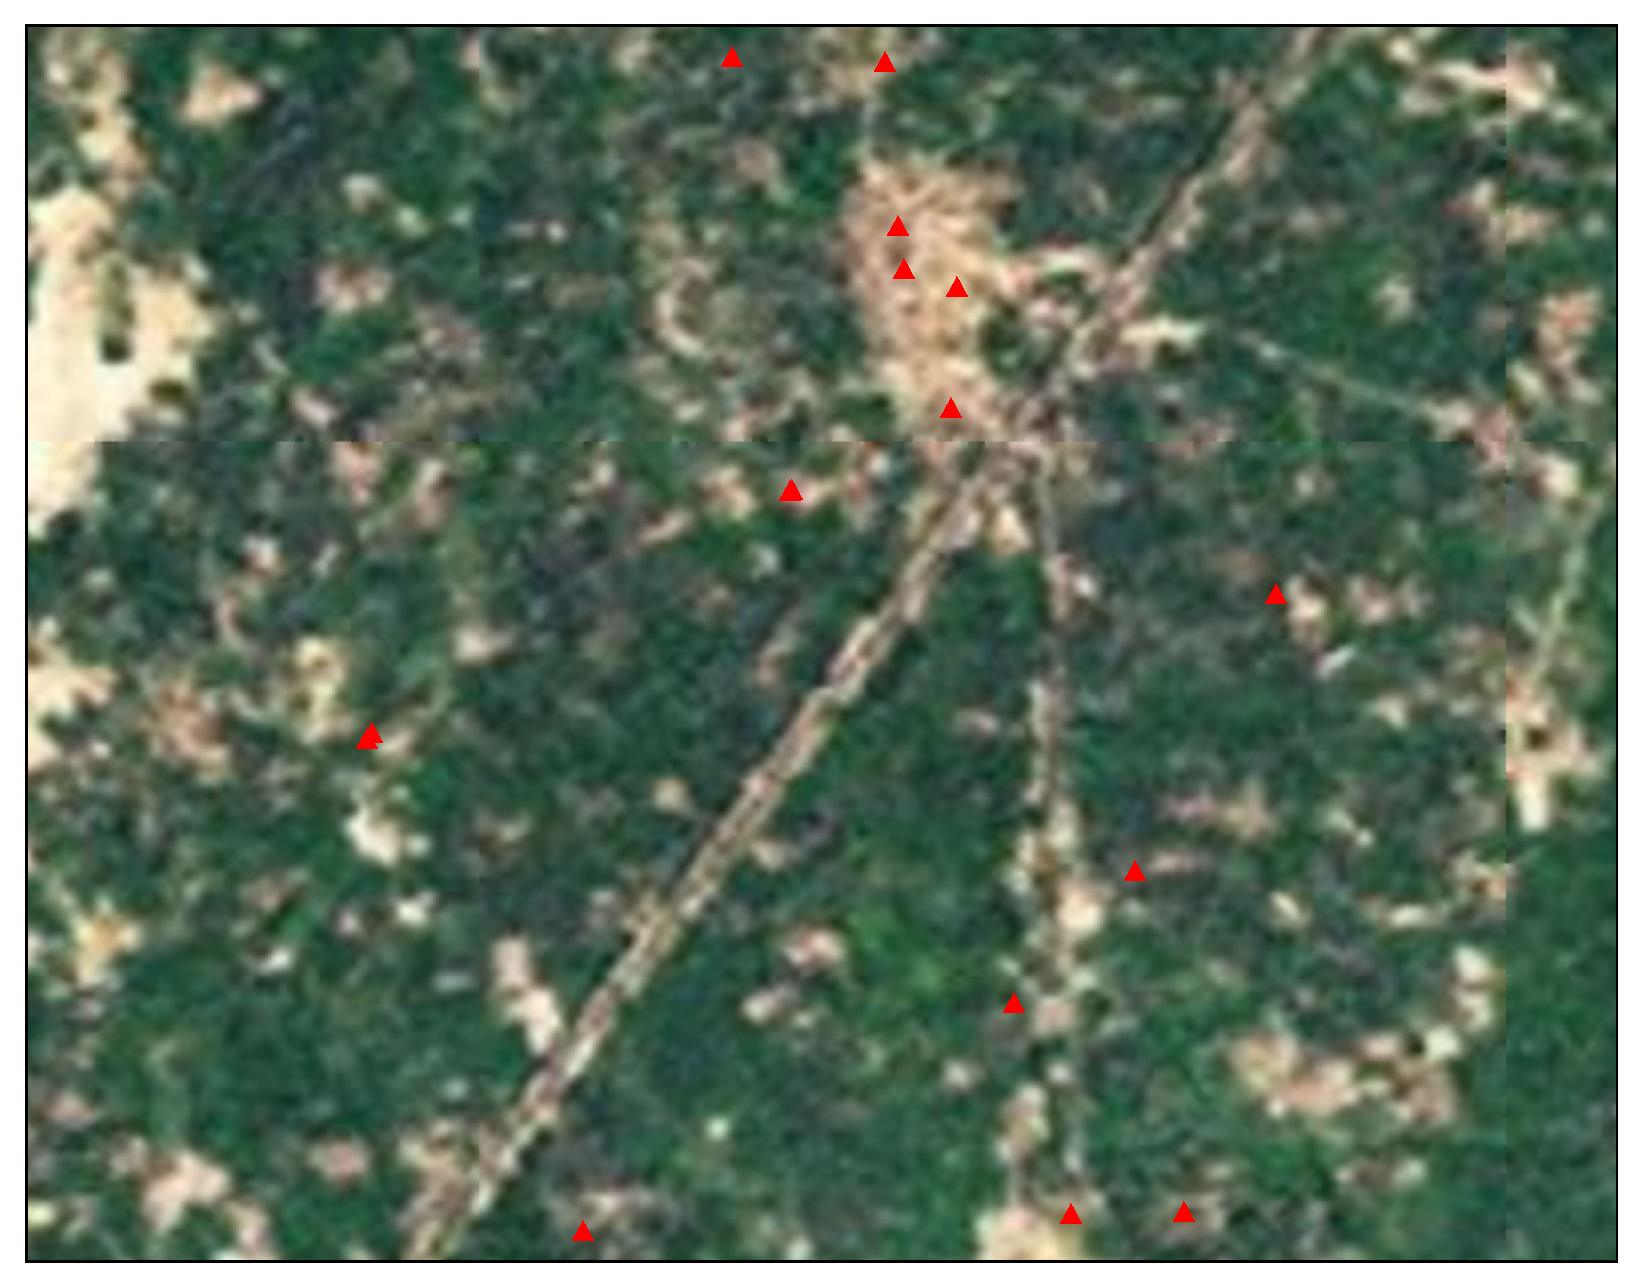
\includegraphics[scale=0.4]{maps/disparate_farming.pdf}
		\end{center}
	\end{figure}
\end{frame}


\begin{frame}{Measuring Learning}
	Lagged-Value-Added Model:	
	\begin{eqnarray}
		Y_{i,t}=\alpha_tX_{i,t}+\alpha_{t-1}X_{i,t-1}+ \dots + \alpha_1X_{i,1} + \epsilon_{i,t}
	\end{eqnarray}
	\pause
	\begin{eqnarray}
		Y_{i,t}=X_{i,t}\alpha+Y_{i,t-1}\beta + \epsilon_{i,t}\label{primary}
	\end{eqnarray}
	\begin{itemize}
		\item Flexible persistence parameter
		\item All past scores included to control of measurement error.
		\pause
		\item Controls for differences in initial levels, but not differences in rates. 
	\end{itemize}
\end{frame}

\begin{frame}{Measuring Learning}
	Village Level:
	\begin{enumerate}
		\item Run Lagged-Value Added regressions with village-school type dummies for each village $j$.
		\begin{eqnarray*}
			Y_{i,t}=X_{i,t}\alpha+Y_{i,t-1}\beta + \mathbb{I}_{i,j,type,t}\gamma_{j, type}+\epsilon_{i,t}
		\end{eqnarray*}
		\item Extract dummies and calculate village public-private gap.
		\item Analyze at level of village.
	\end{enumerate}
	\begin{eqnarray*}
		Gap_{j}=Z_{j}\delta+\eta_{j}\label{villagespecification}
	\end{eqnarray*}
\end{frame} 

\begin{frame}{Measuring Learning}
	Teacher Level:
	\begin{enumerate}
		\item Run Lagged-Value Added regressions with teacher fixed effects dummies for each teacher $k$.
		\begin{eqnarray*}
			Y_{i,t}=X_{i,t}\alpha+Y_{i,t-1}\beta + \mathbb{I}_{i,k,t}\zeta_{k}+\epsilon_{i,t}\label{teacherspecification}
		\end{eqnarray*}
		
		\item Extract fixed effect coefficients as estimates of teacher contributions
		\item Analyze at level of teacher (weighted by number of students).
	\end{enumerate}
\end{frame}


\section{Fractionalization and Performance}\label{}
\begin{frame}{Outline}
	\tableofcontents[currentsection]
\end{frame}

% \begin{frame}{Caste in Punjab}
% \begin{itemize}
% 	\item Very similar to caste in India
% 	\begin{itemize}
% 		\item Biraderi implies ``an inherent, inbuilt hierarchy that governs social interactions''\citep[p. 29]{Gazdar:2007vt}.	
% 	\end{itemize}
% 	\item Not synonymous with economic status:
% 	\begin{itemize}
% 		\item ``the poorest Jatt is still better off than the richest kammi.'' \citep[p. 13]{Gazdar:2007vt} 
% 	\end{itemize}
% \end{itemize}
% \end{frame}
	
\begin{frame}{Caste in Punjab}
	\begin{figure}[htb]
		\begin{center}
		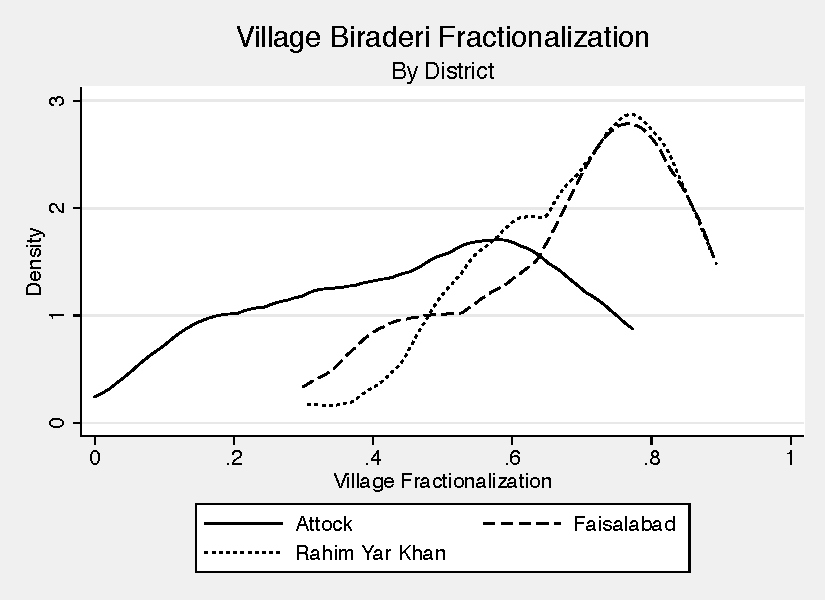
\includegraphics[scale=0.6]{graphs/village_frac_by_district.pdf}
		\end{center}
	\end{figure}		
\end{frame}


\begin{frame}{}
	\begin{figure}[h]
		\centering	
		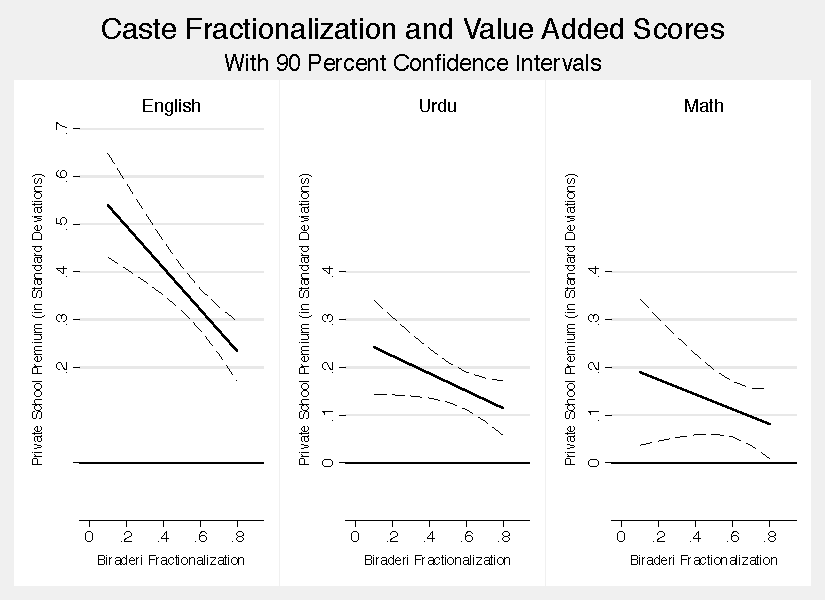
\includegraphics[scale=0.8]{graphs/kids_combined.pdf}
	\end{figure}
\end{frame}

\begin{frame}{}
	\begin{figure}[htb]
		\begin{center}
		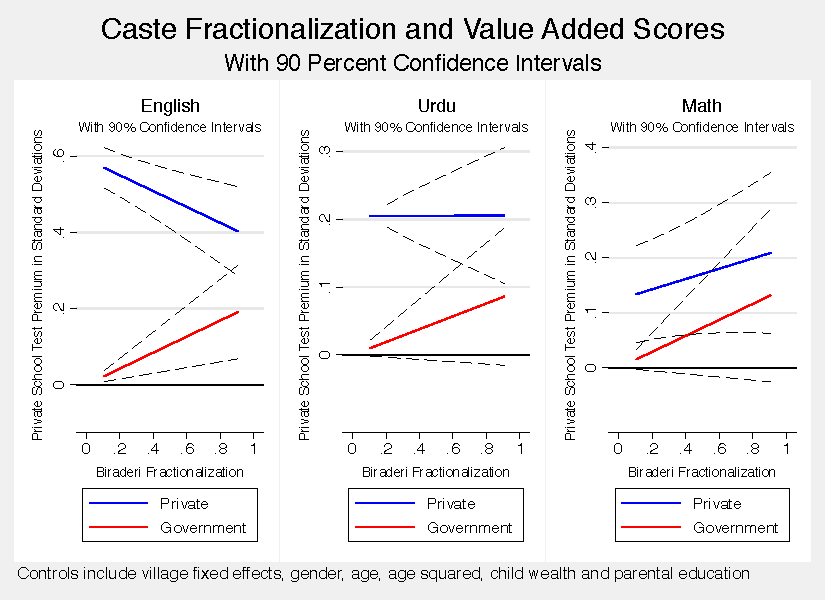
\includegraphics[scale=0.8]{graphs/kids_combined_district.pdf}
		\end{center}
	\end{figure}
	
\end{frame}

\section{Teaching Quality}\label{}
\begin{frame}{Outline}
	\tableofcontents[currentsection]
\end{frame}

\begin{frame}{No Difference in Inputs}
	\begin{figure}[htb]
		\begin{center}
		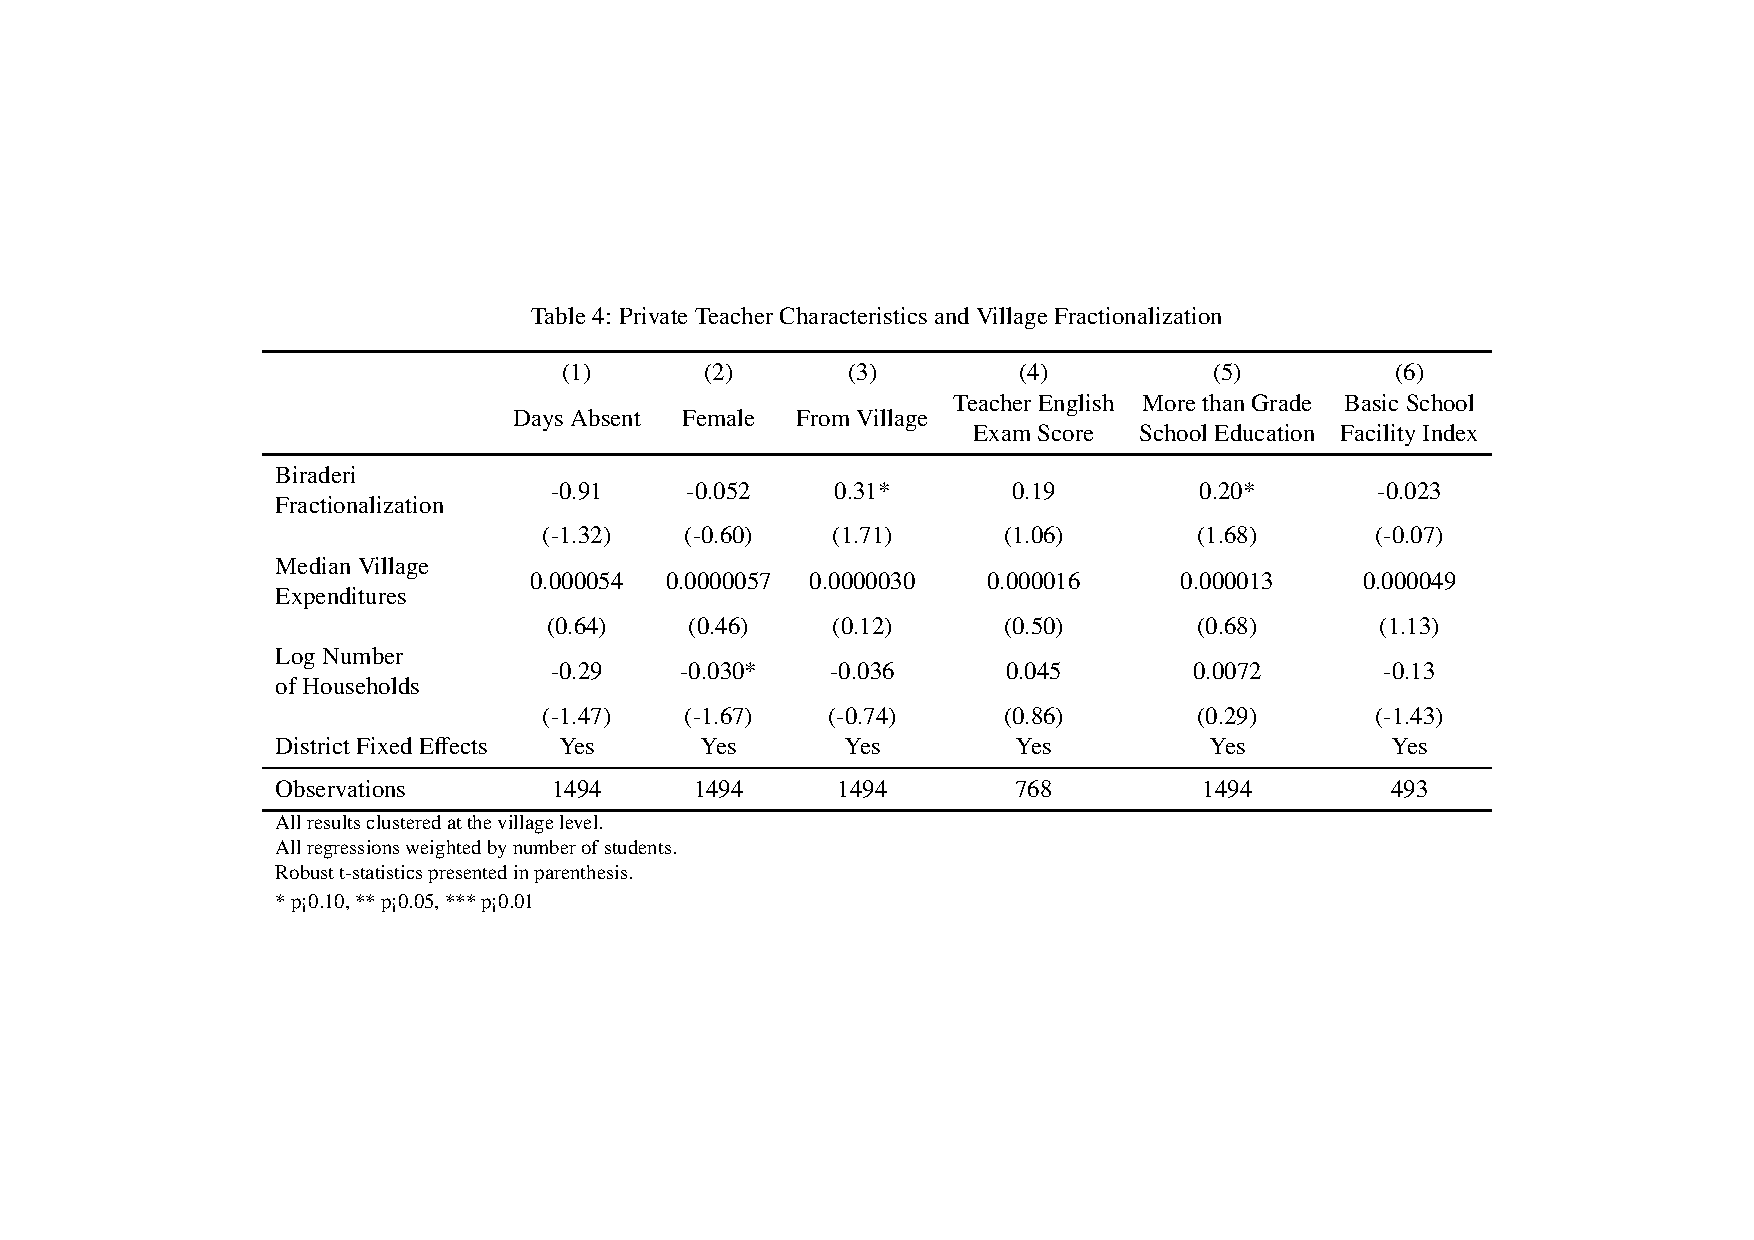
\includegraphics[scale=0.5]{tables/Private_teacher_quality.pdf}
		\end{center}
	\end{figure}
\end{frame}

\begin{frame}{No Difference in Inputs}
	\begin{figure}[htb]
		\begin{center}
		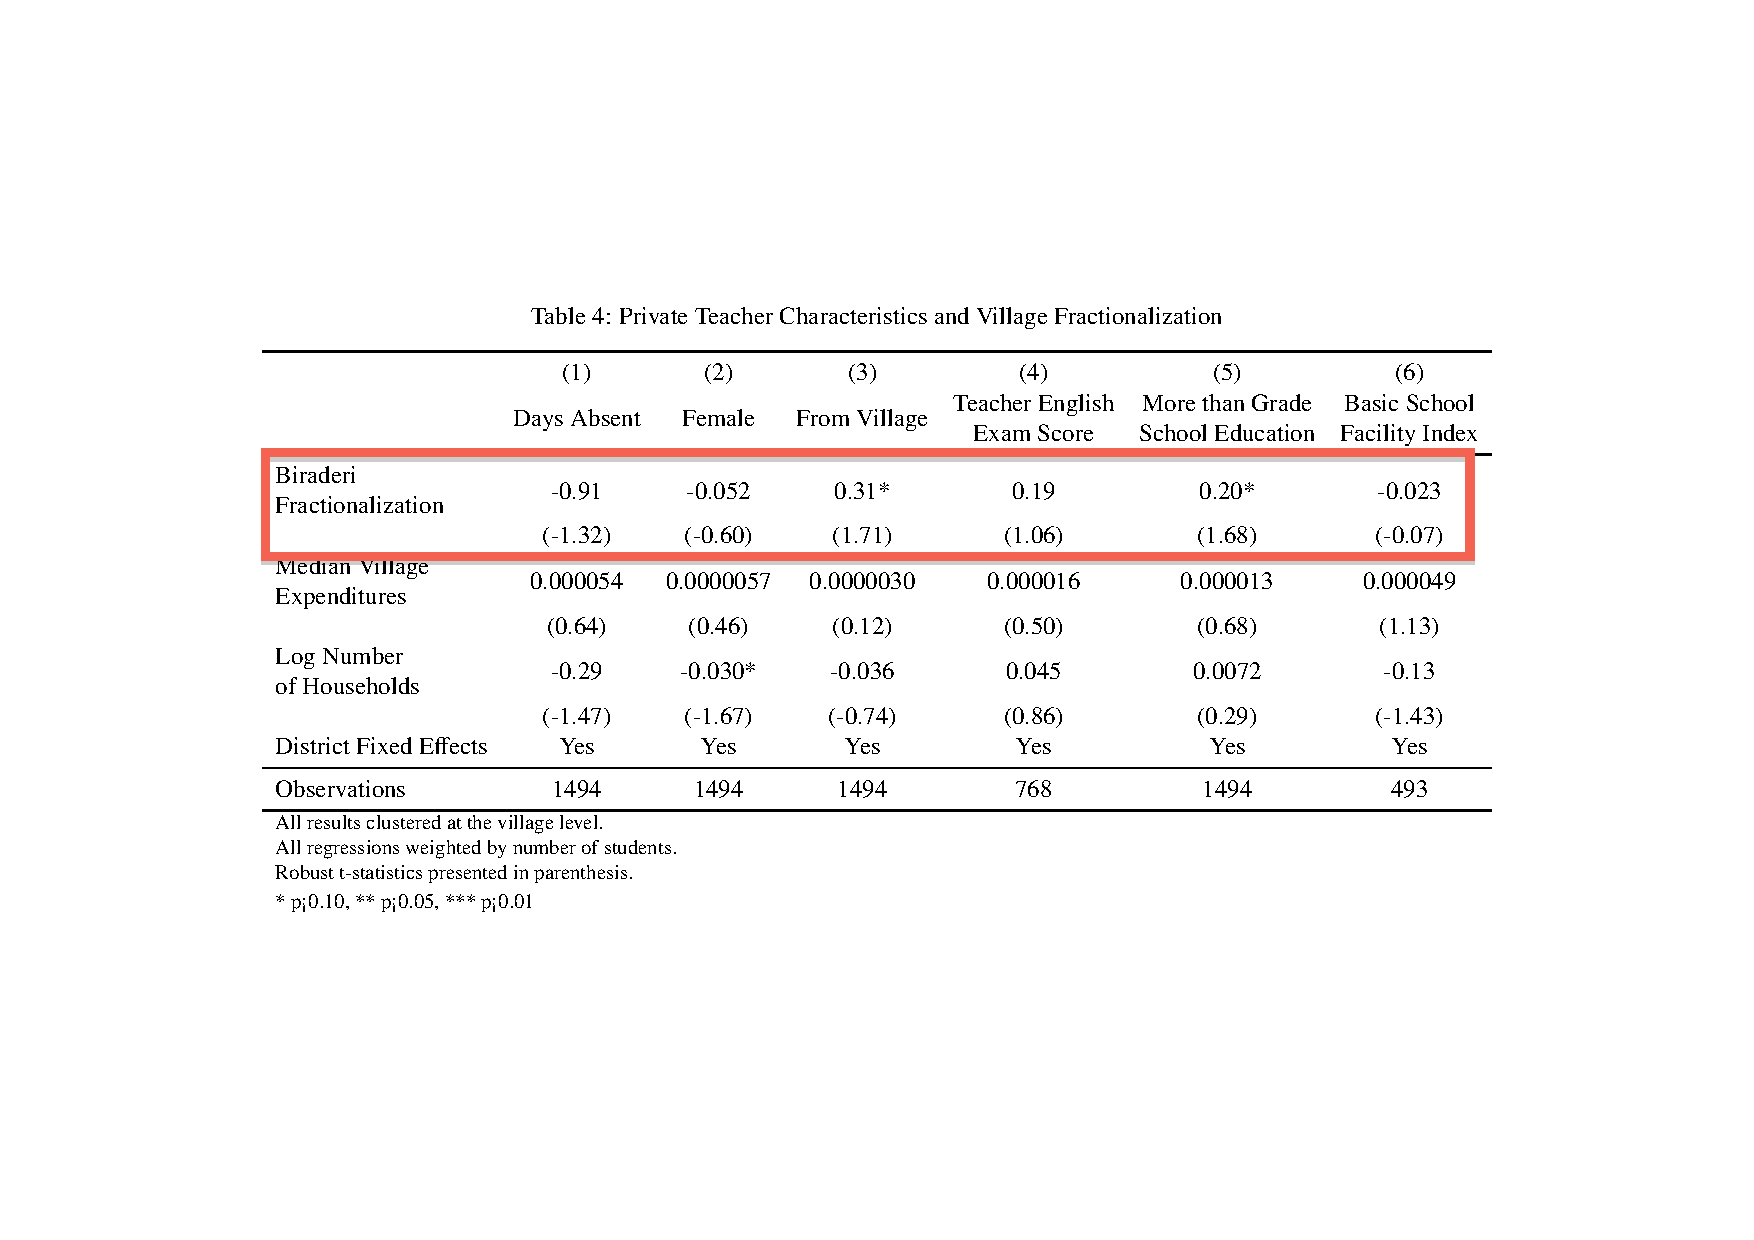
\includegraphics[scale=0.5]{tables/Private_teacher_quality_box1.pdf}
		\end{center}
	\end{figure}
\end{frame}


\begin{frame}{No Difference in Inputs}
	\begin{figure}[htb]
		\begin{center}
		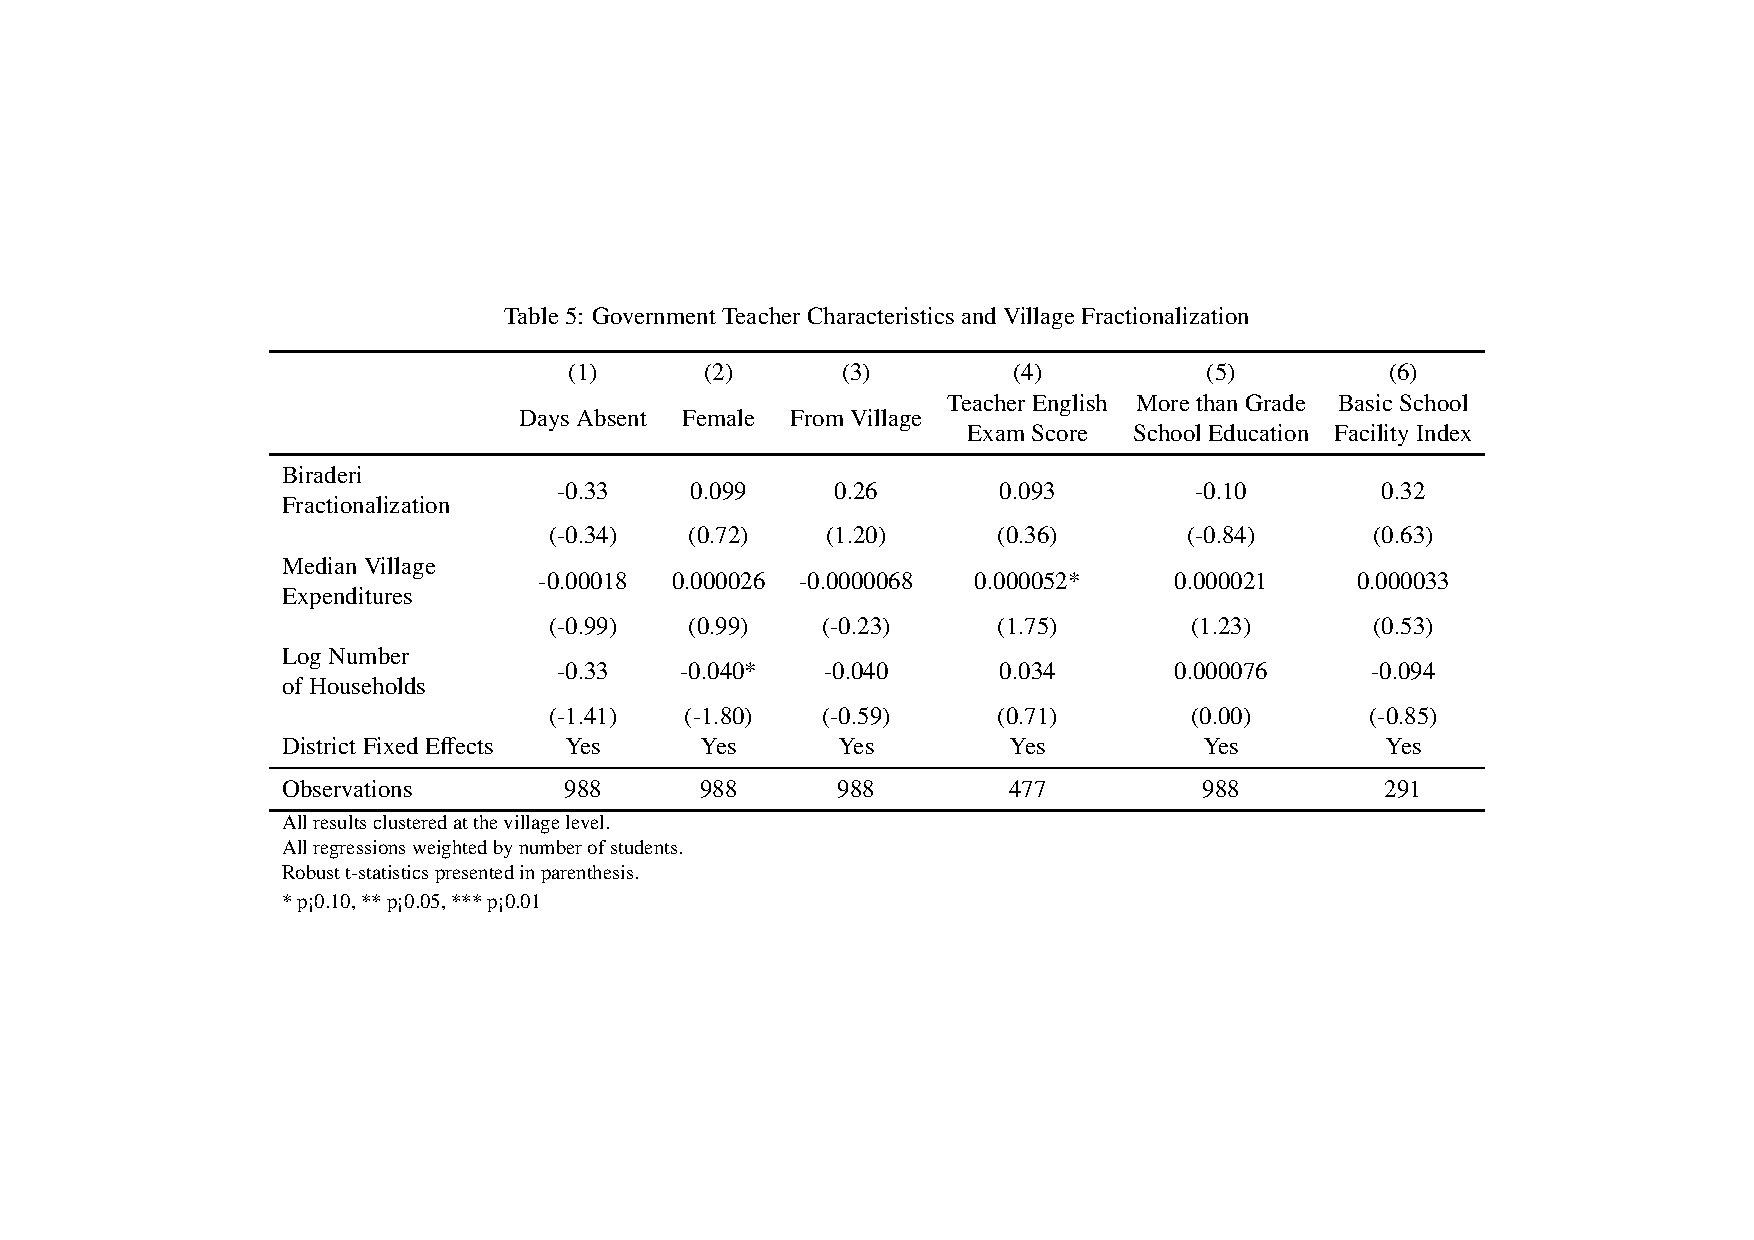
\includegraphics[scale=0.5]{tables/govt_teacher_quality.pdf}
		\end{center}
	\end{figure}	
\end{frame}


\begin{frame}{No Difference in Inputs}
	\begin{figure}[htb]
		\begin{center}
		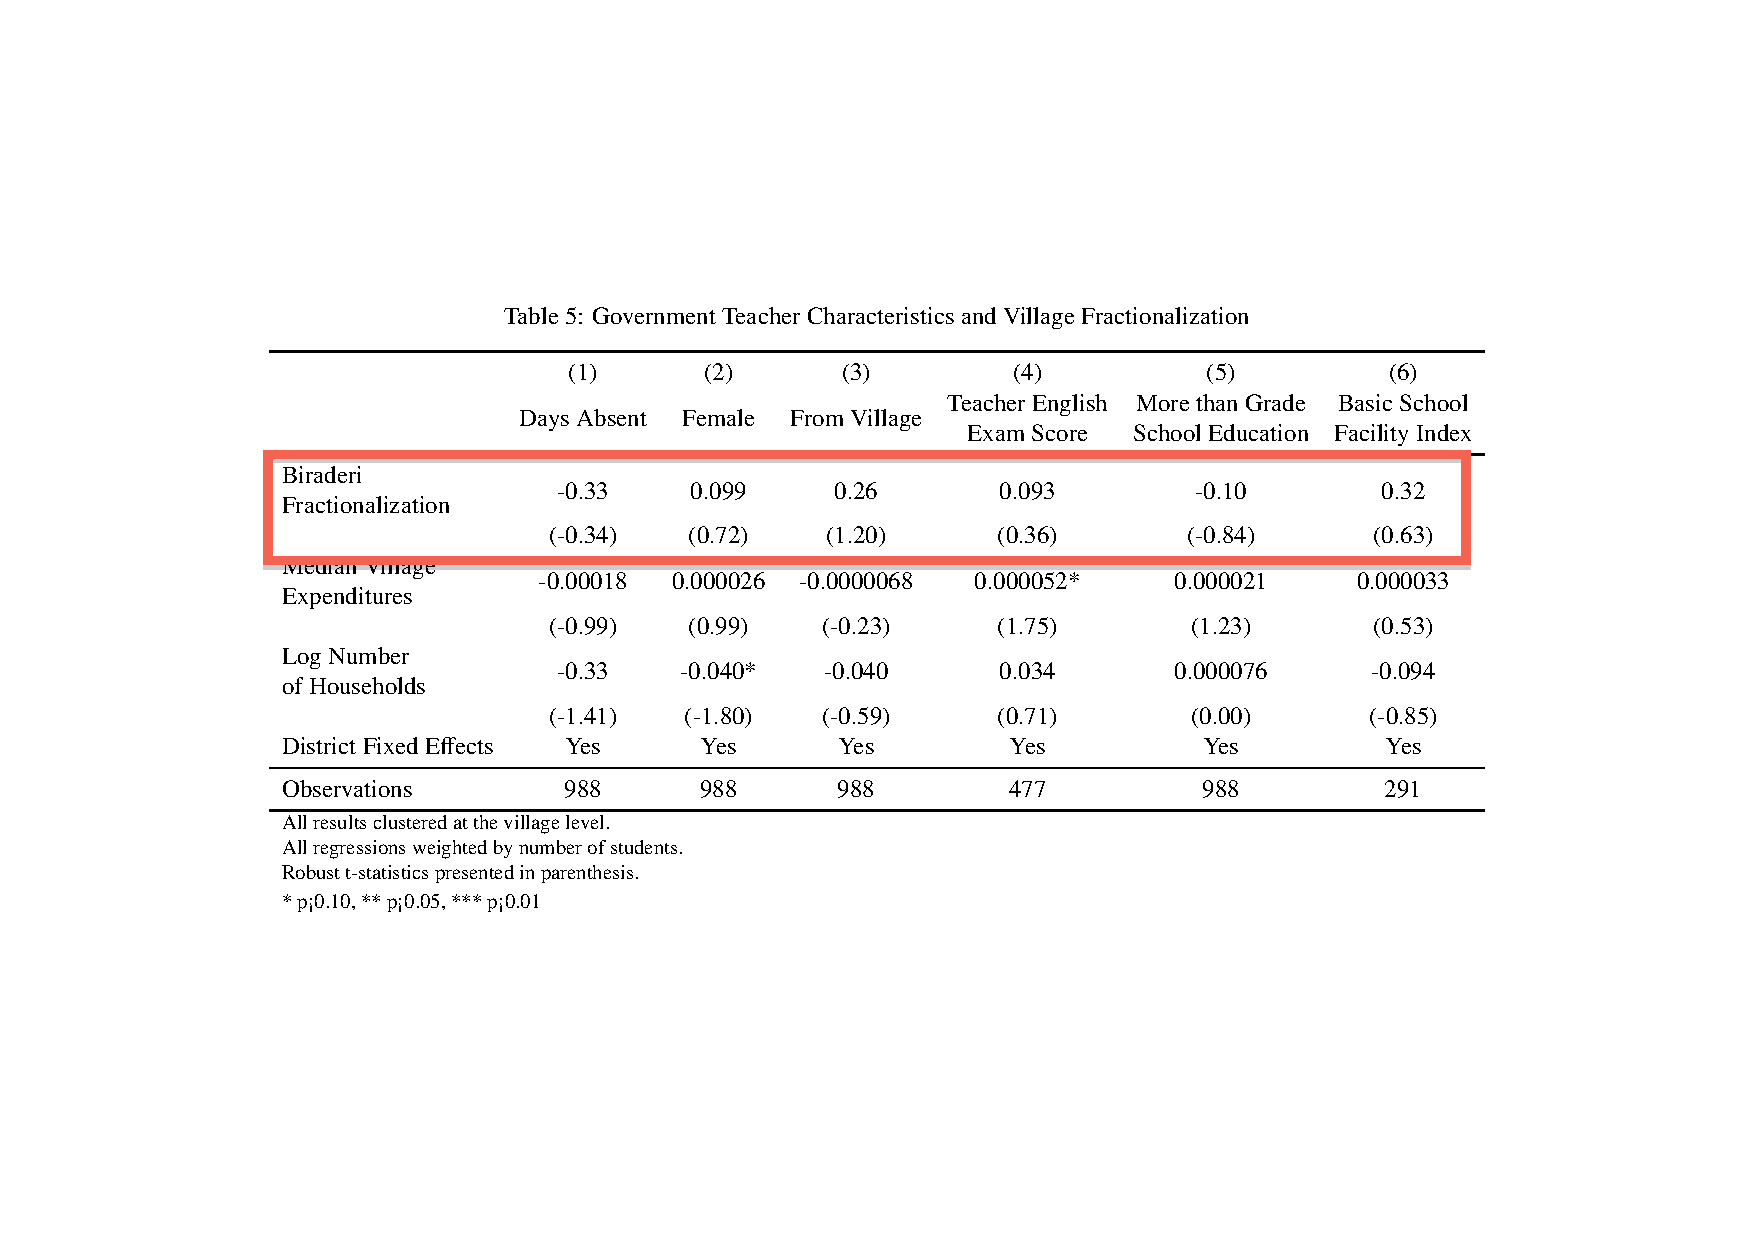
\includegraphics[scale=0.5]{tables/govt_teacher_quality_box1.pdf}
		\end{center}
	\end{figure}
\end{frame}


\begin{frame}{}
	\begin{figure}[htb]
		\begin{center}
		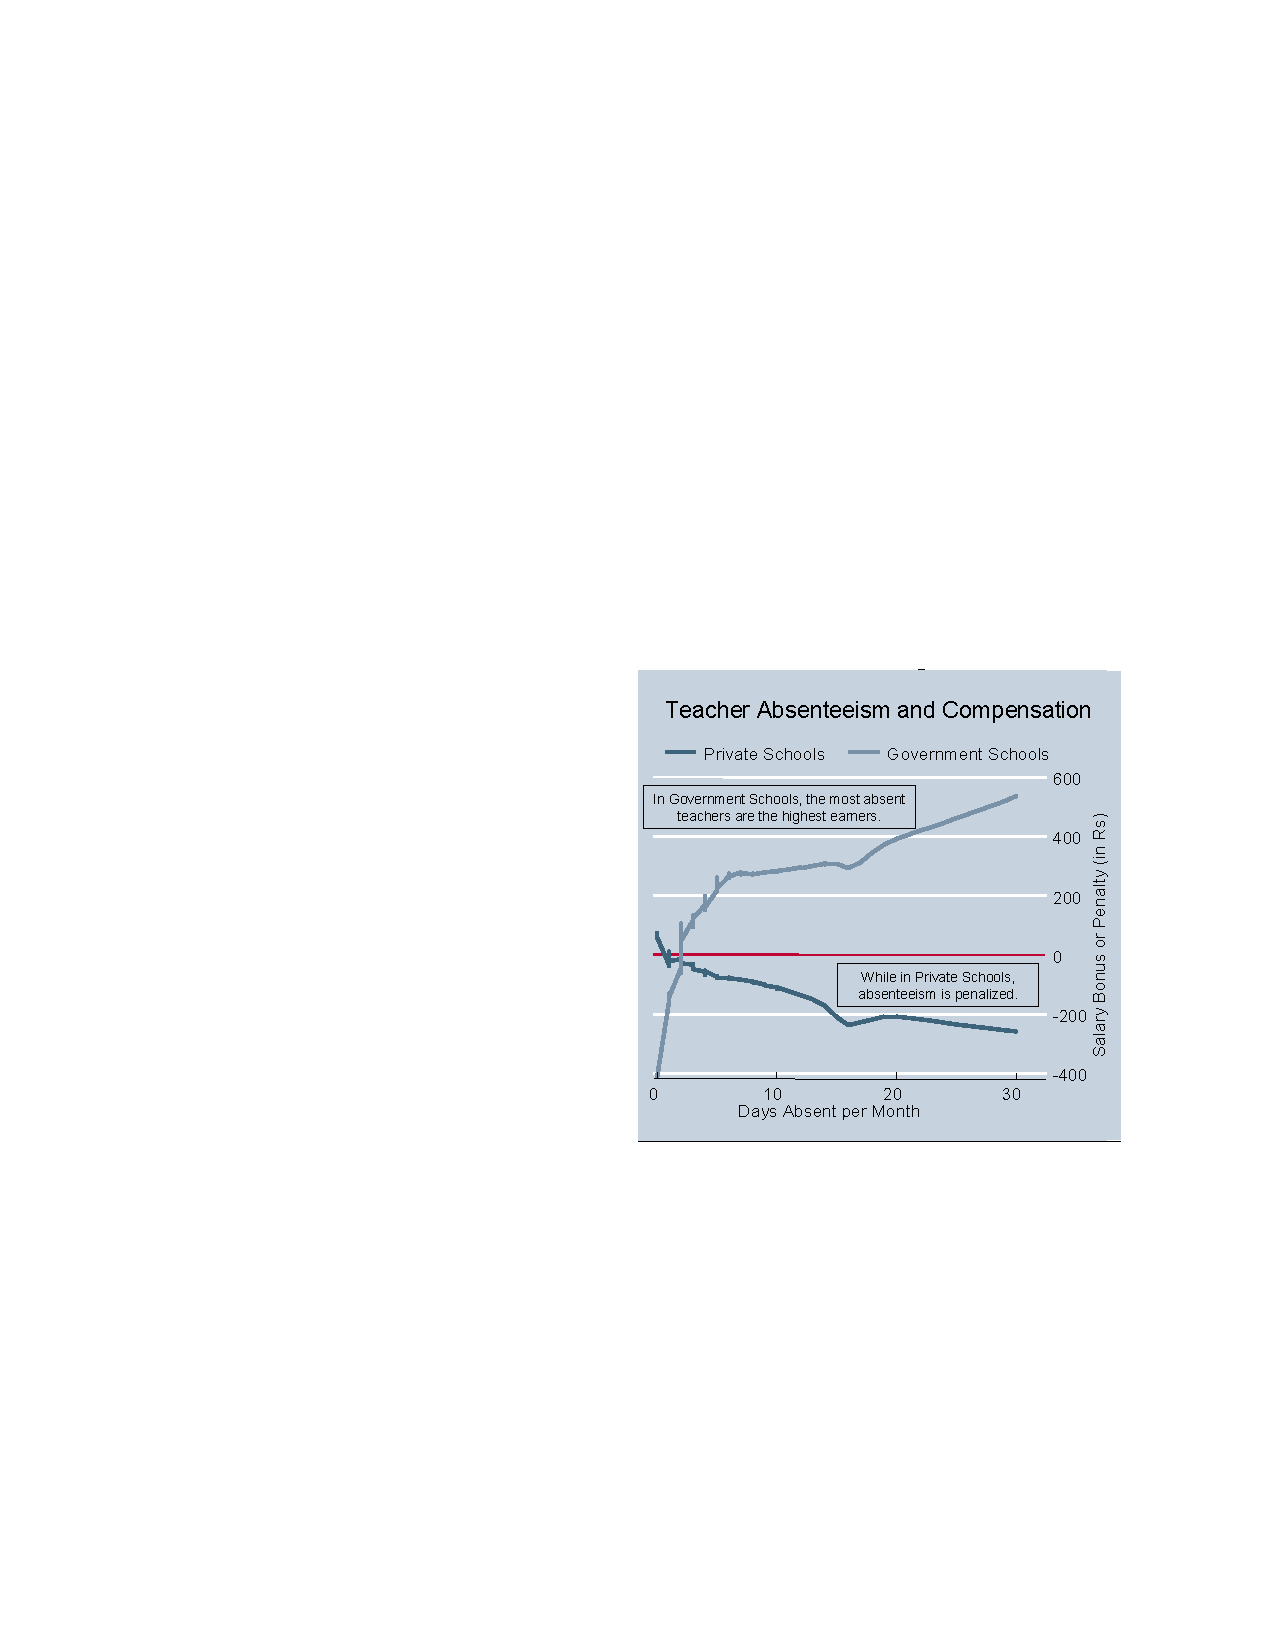
\includegraphics[scale=1.1]{graphs/absenteeism_and_pay.pdf} 
		\end{center}
	\end{figure}
\end{frame}

\begin{frame}{}
	\begin{figure}[htb]
		\begin{center}
			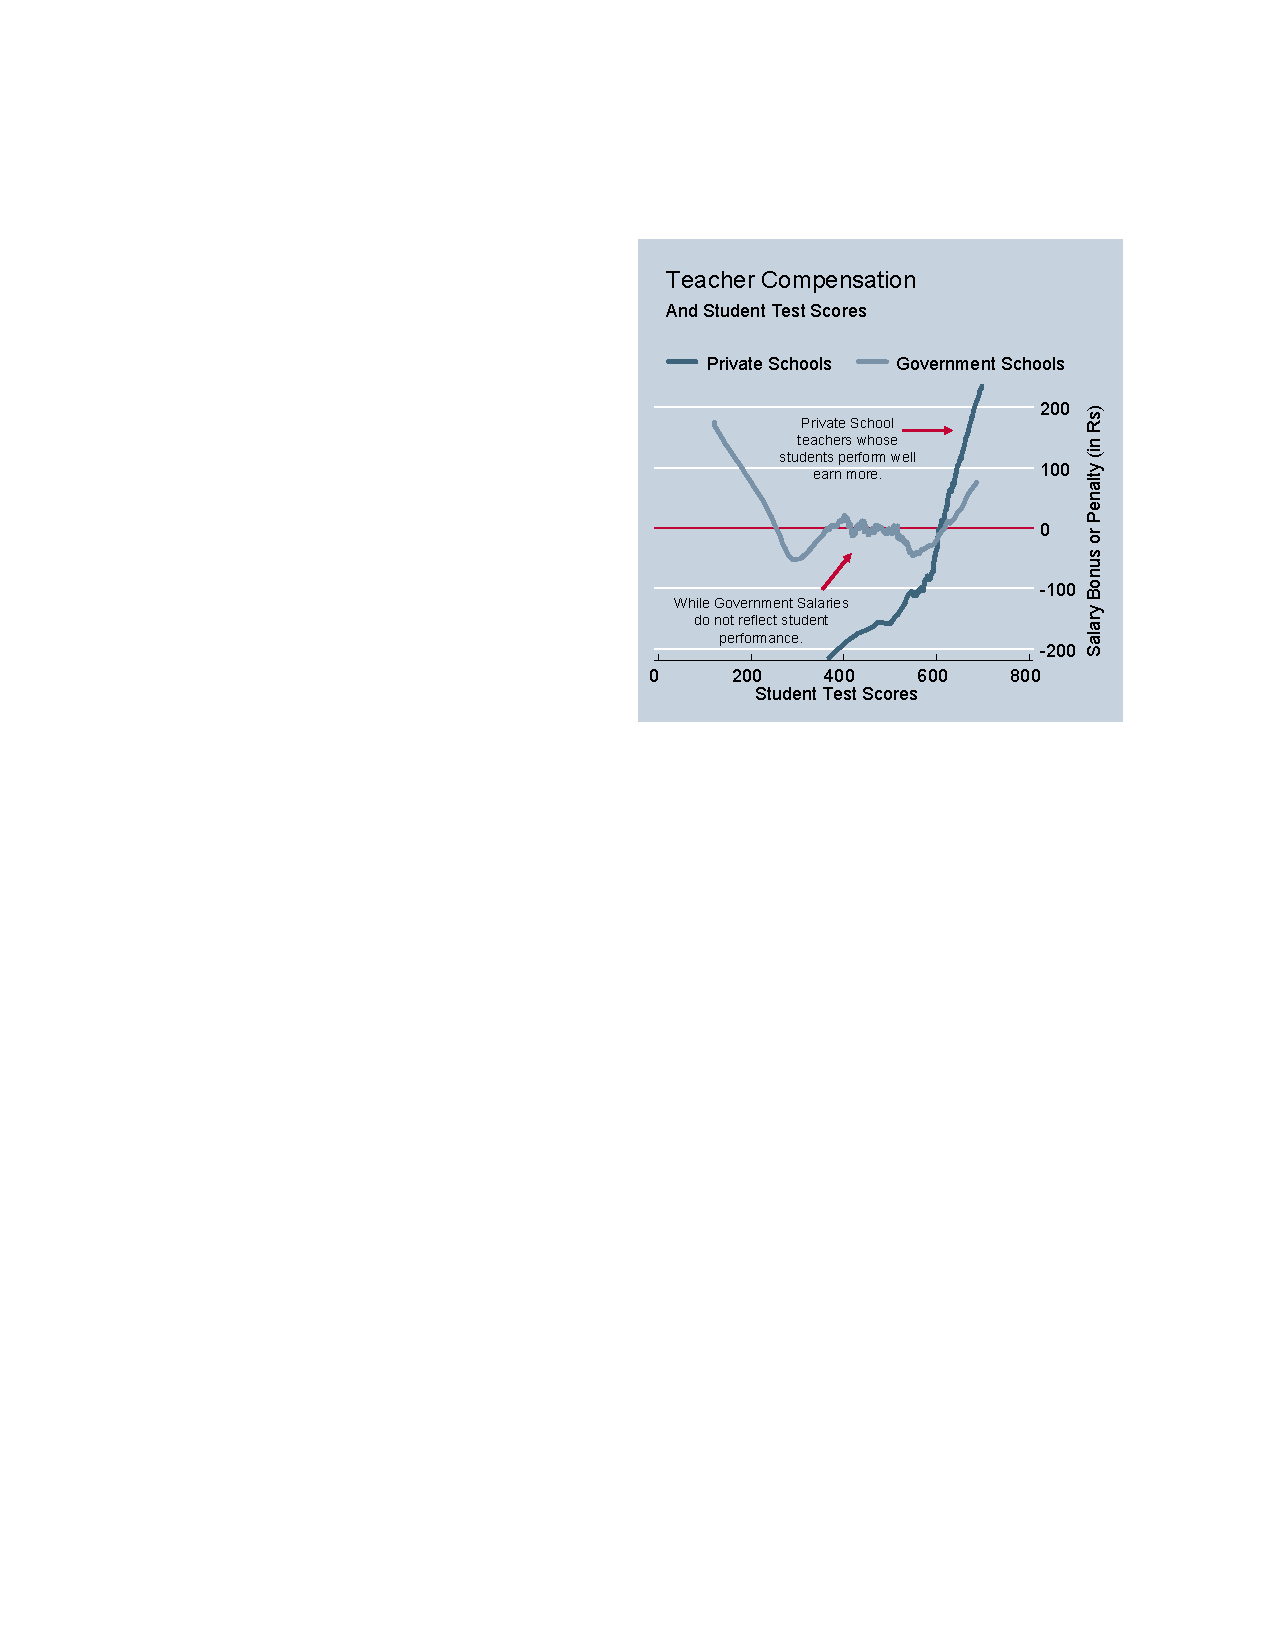
\includegraphics[scale=1.1]{graphs/compensation_scores.pdf}
		\end{center}
	\end{figure}
\end{frame}

\begin{frame}{}
\begin{figure}[htb]
	\begin{center}
	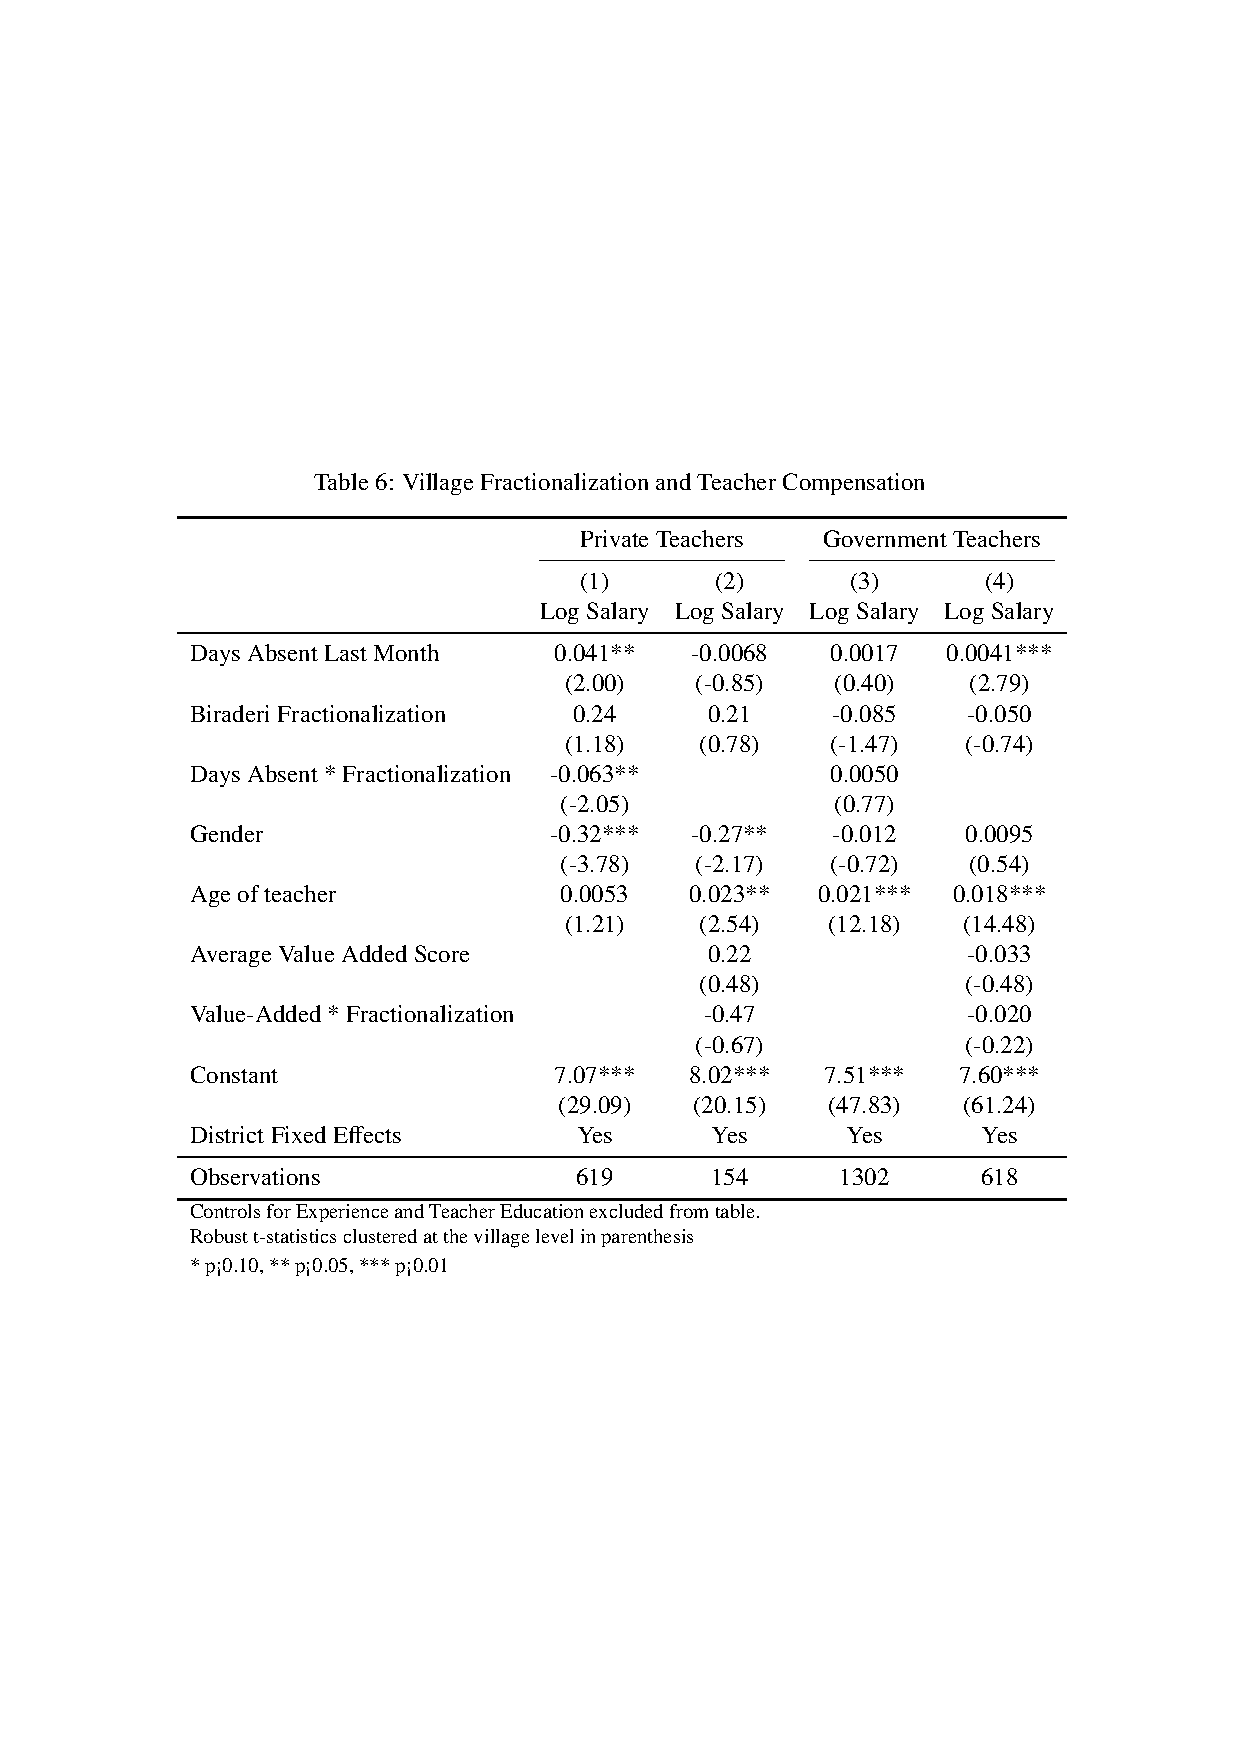
\includegraphics[scale=0.65]{tables/frac_and_compensation.pdf}
	\end{center}
\end{figure}
\end{frame}

\begin{frame}{}
\begin{figure}[htb]
	\begin{center}
	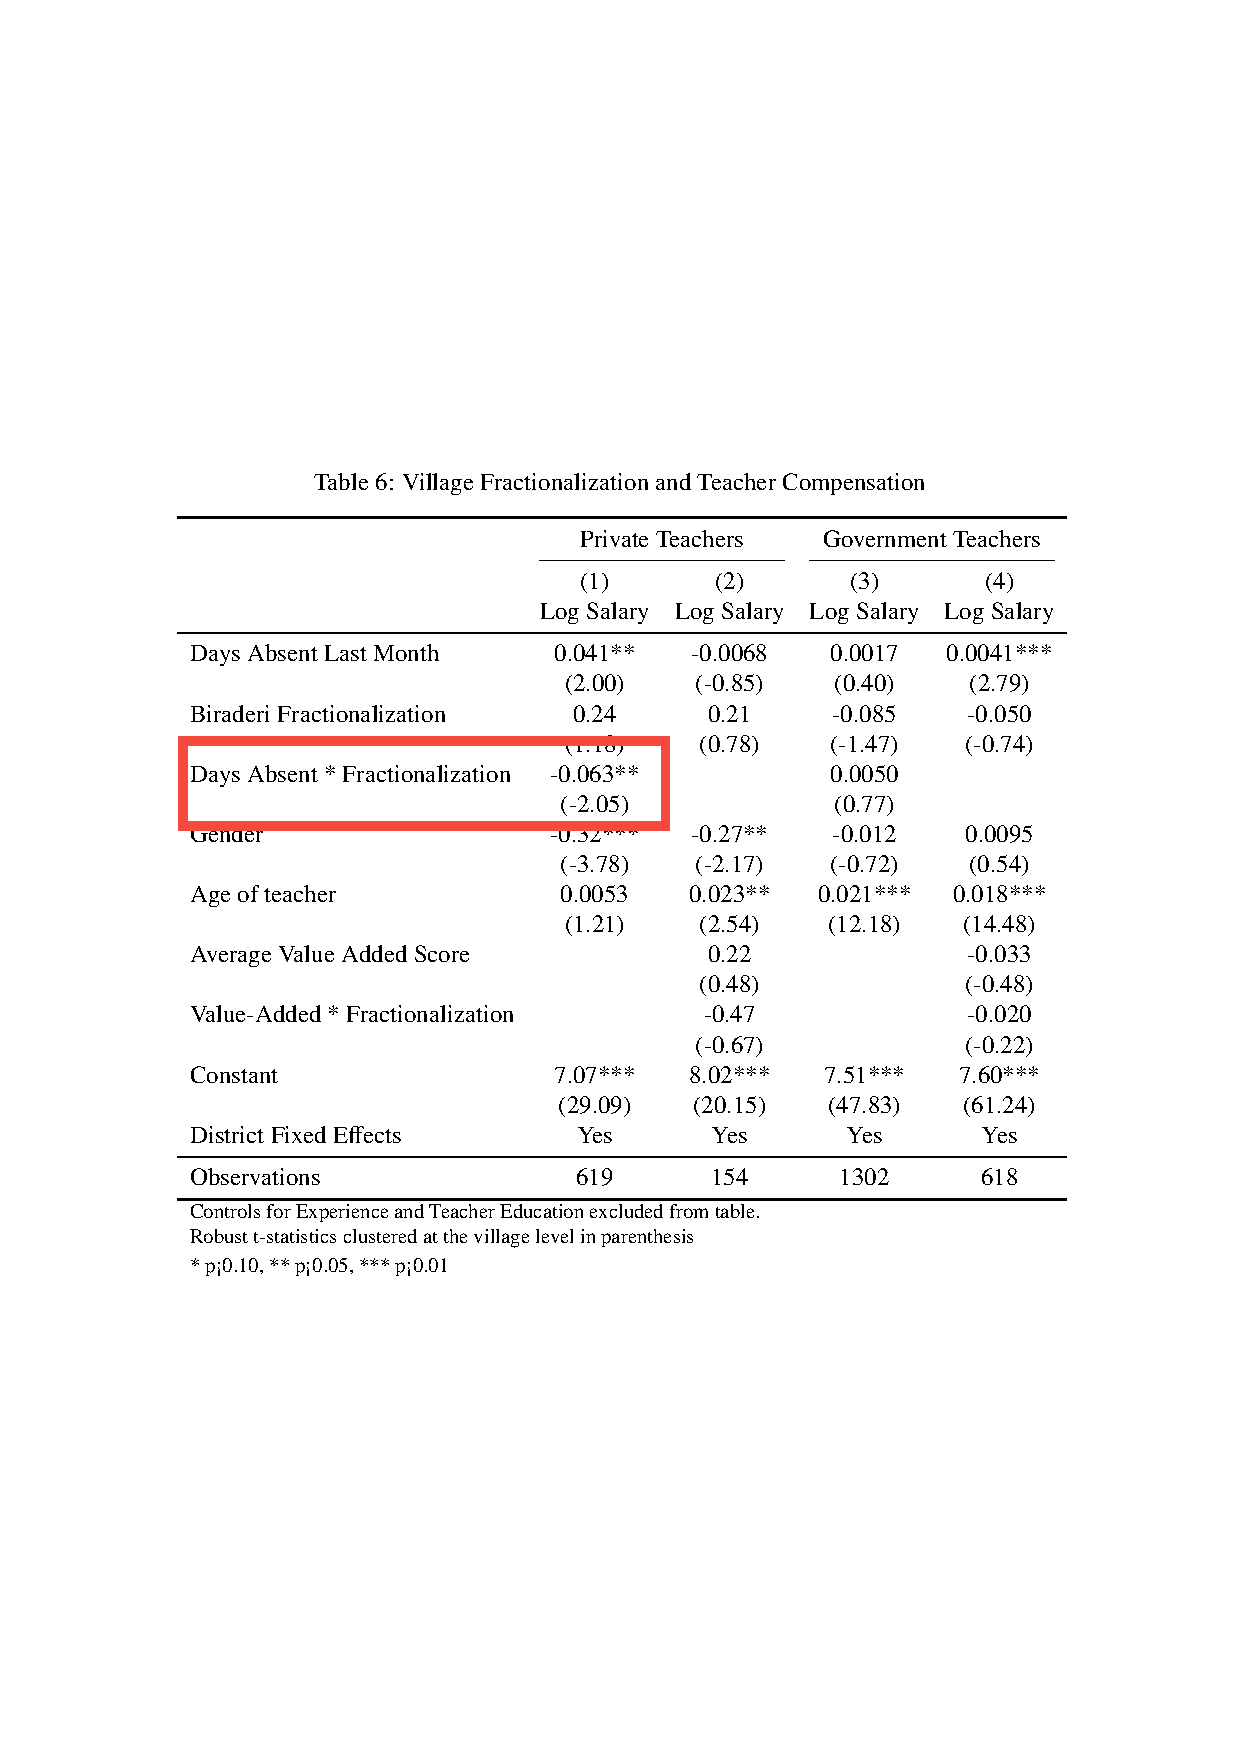
\includegraphics[scale=0.65]{tables/frac_and_compensation_box1.pdf}
	\end{center}
\end{figure}
\end{frame}

\begin{frame}{}
\begin{figure}[htb]
	\begin{center}
	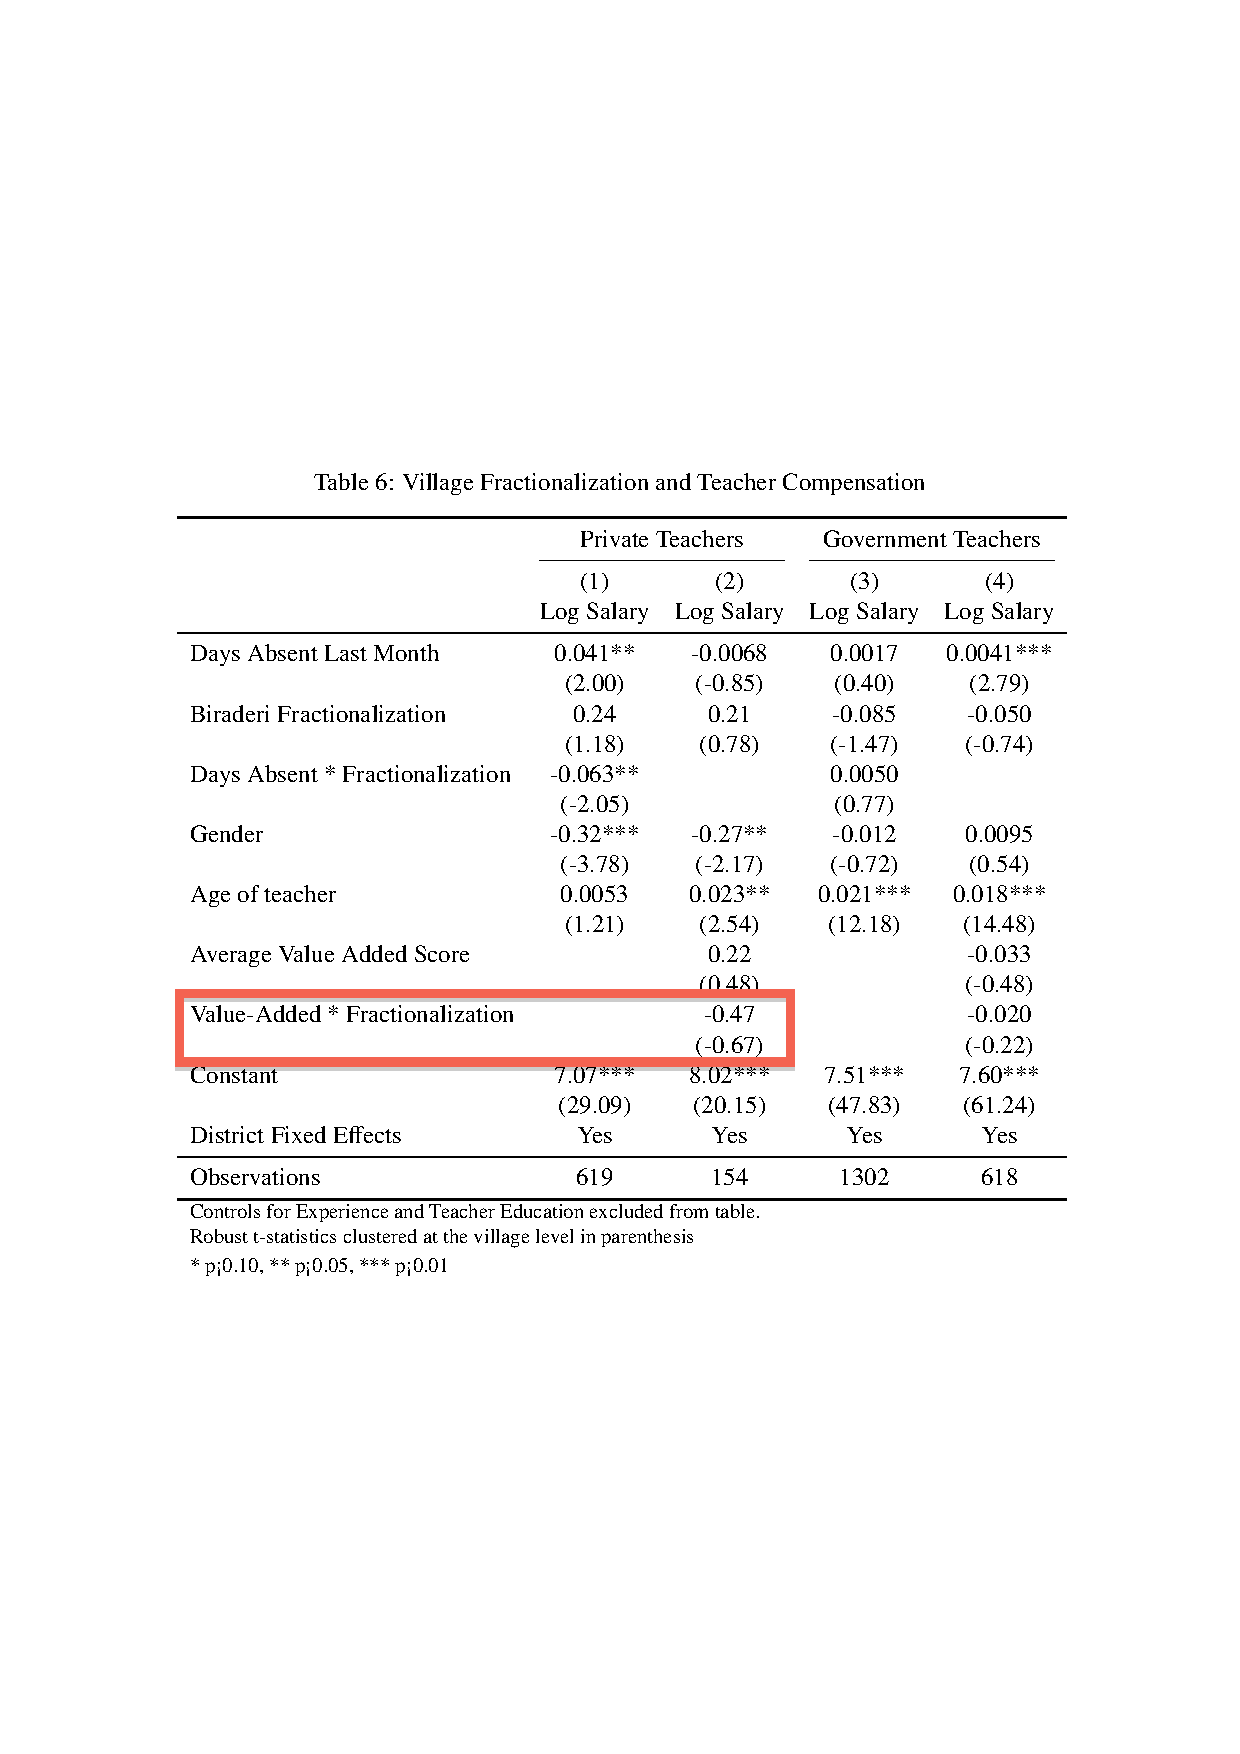
\includegraphics[scale=0.65]{tables/frac_and_compensation_box2.pdf}
	\end{center}
\end{figure}
\end{frame}

\begin{frame}{}
\begin{figure}[htb]
	\begin{center}
	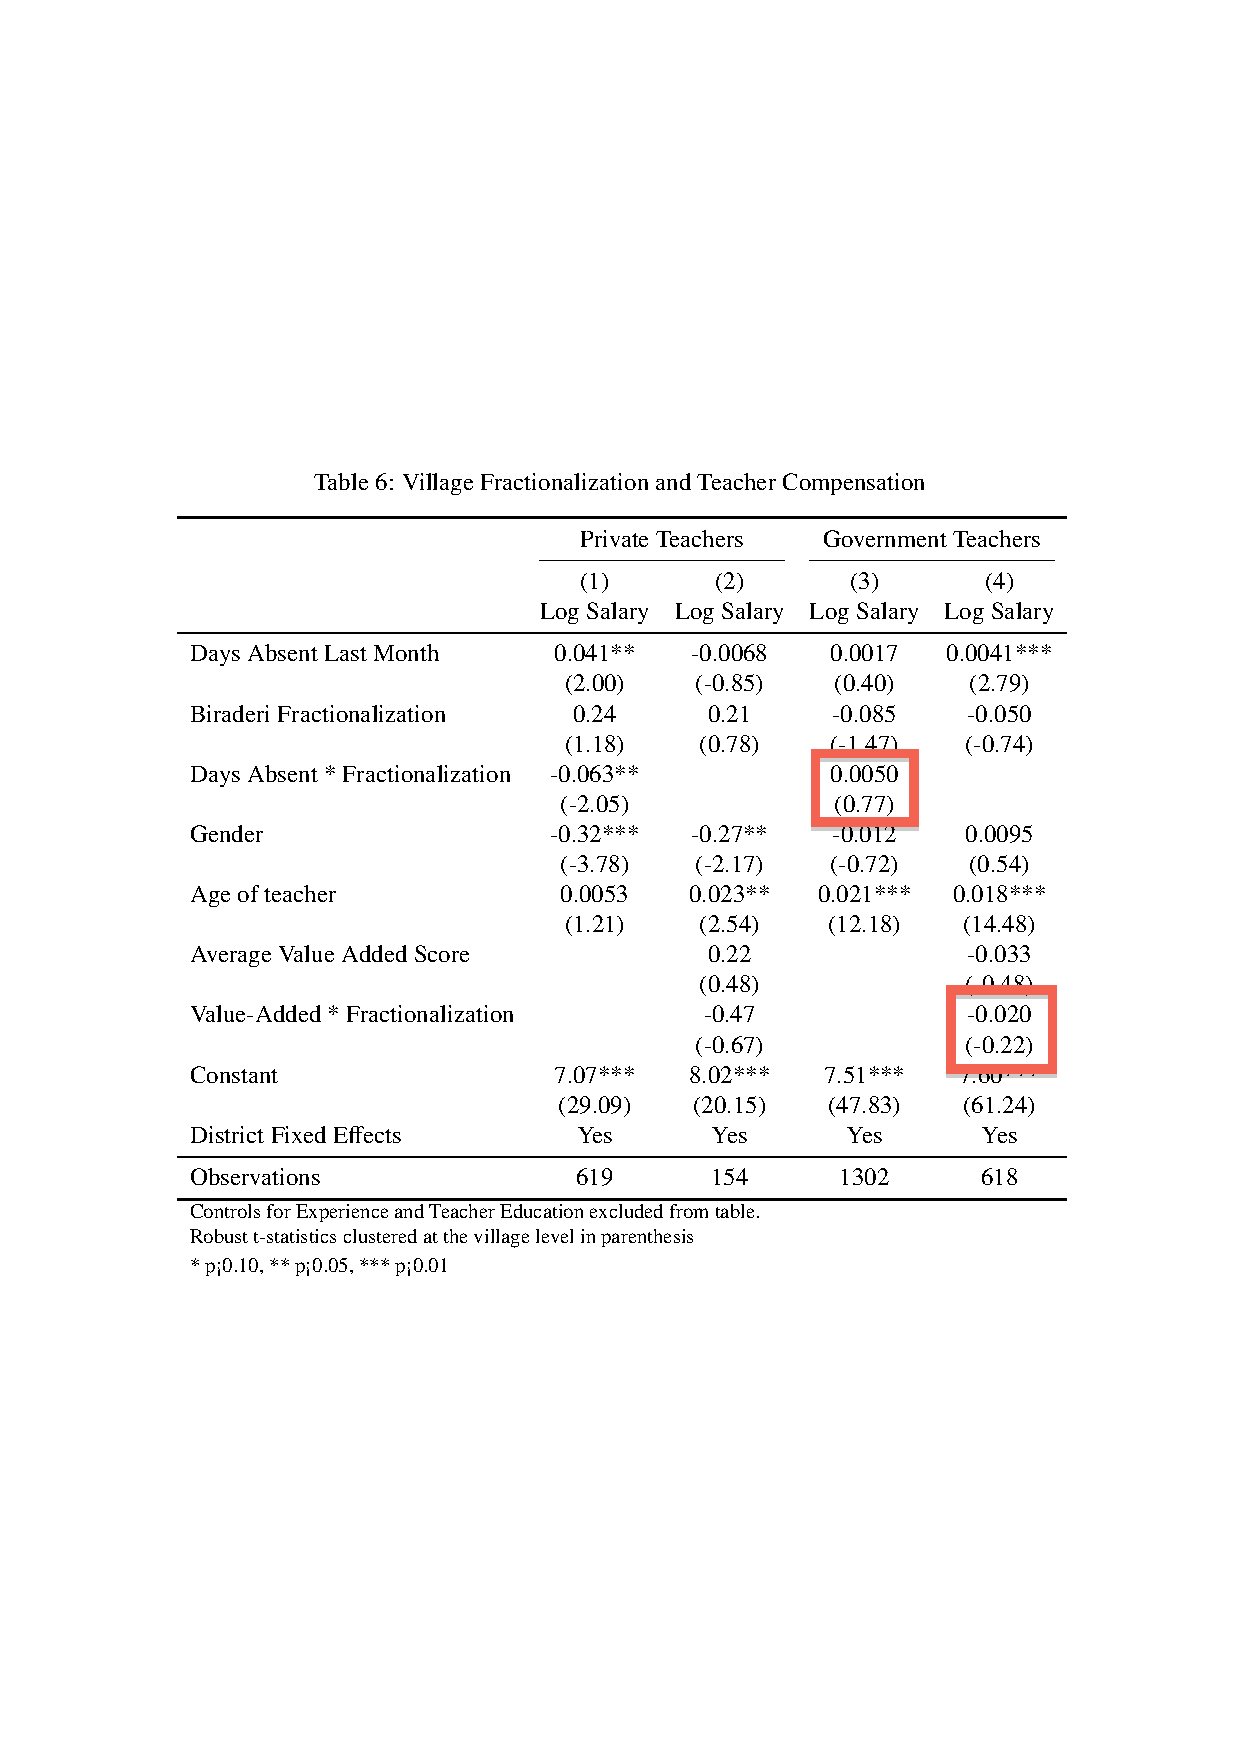
\includegraphics[scale=0.65]{tables/frac_and_compensation_box3.pdf}
	\end{center}
\end{figure}
\end{frame}


\section{Selective Sorting}\label{}
\begin{frame}{Outline}
	\tableofcontents[currentsection]
\end{frame}


\begin{frame}{A Sorting Story}
	\begin{description}
		\item [Homogenous Villages:] Children sort on academic potential.
		\item [Fractionalized Villages:] Children also sort by social status.
	\end{description}
	\pause
	\begin{enumerate}
		\item Parents pick winners
	\end{enumerate}
\end{frame}

\begin{frame}{Sorting}
	\begin{figure}[htb]
		\begin{center}
		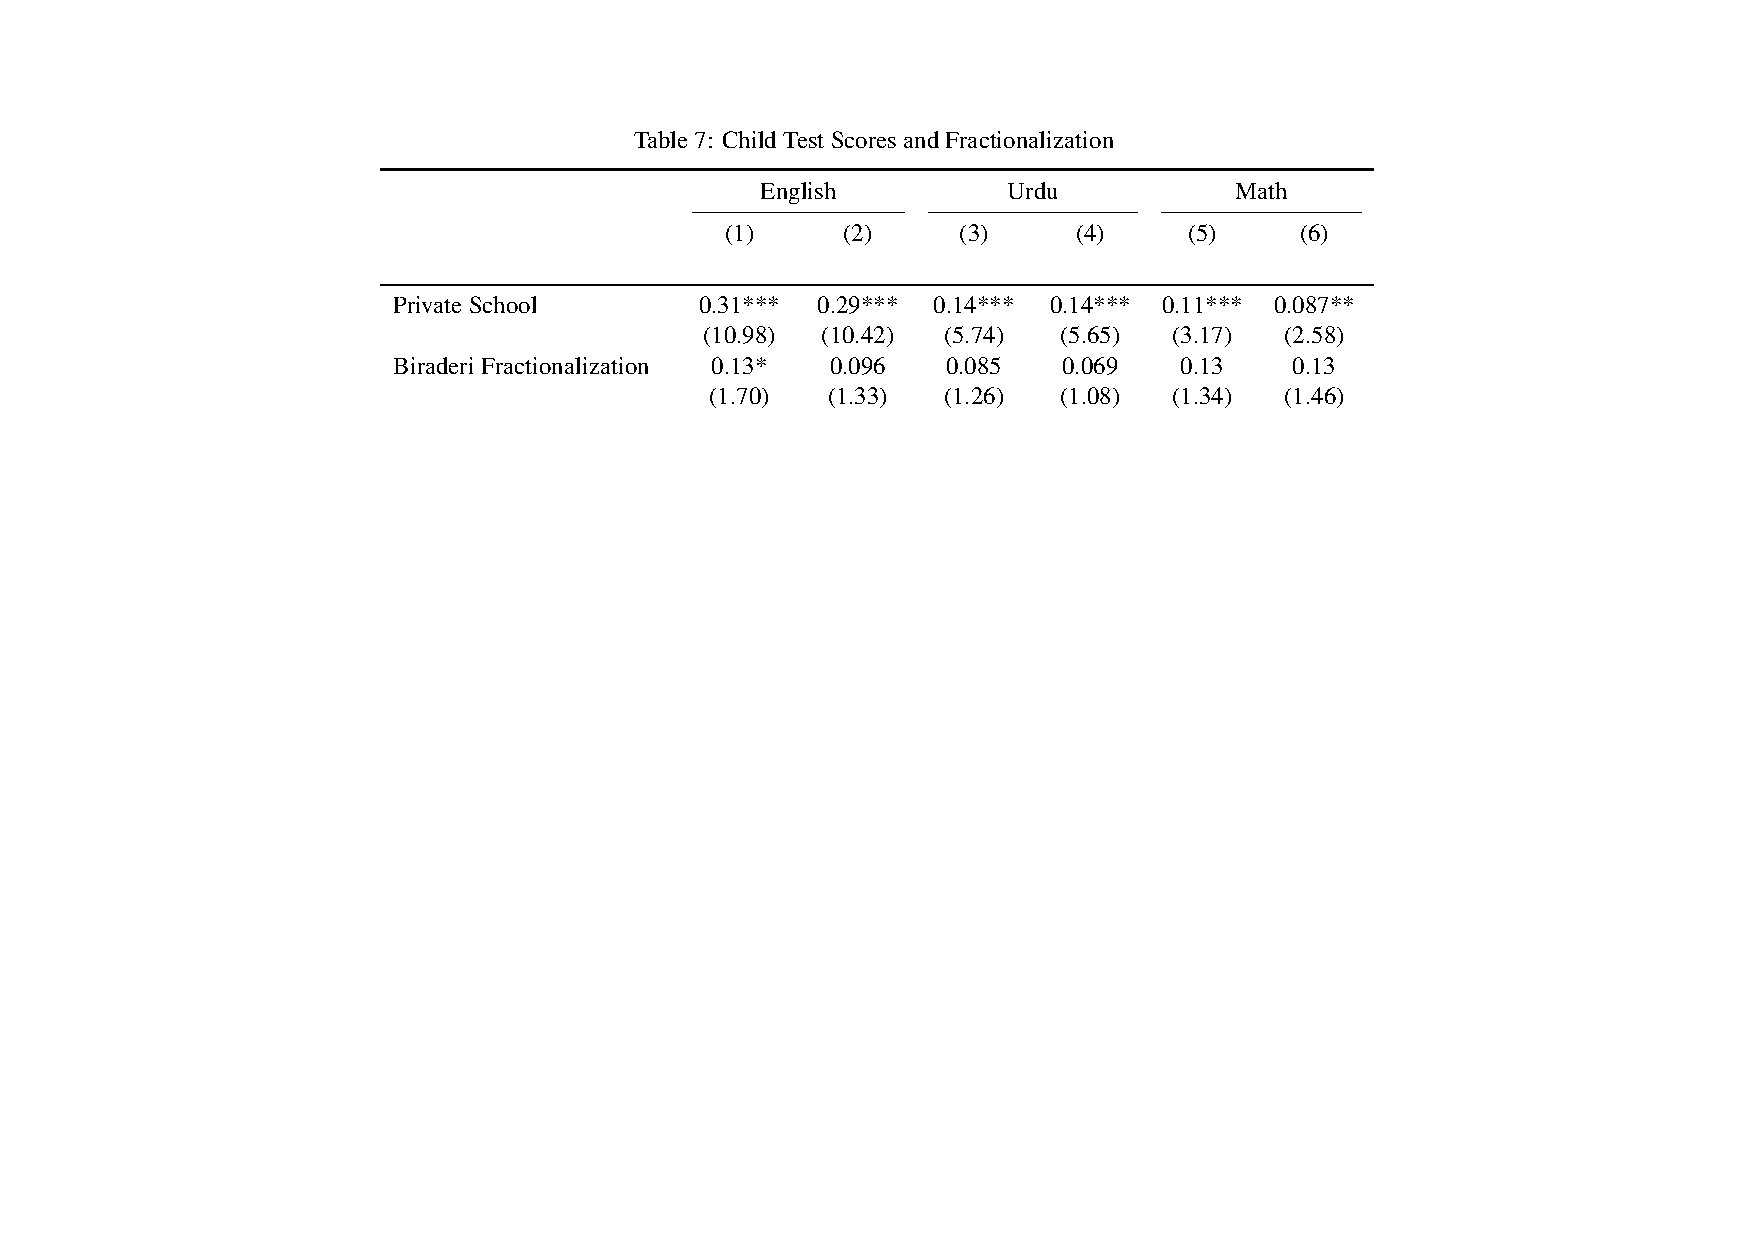
\includegraphics[scale=0.65]{tables/mean_preserving.pdf}
		\end{center}
	\end{figure}
\end{frame}

\begin{frame}{Sorting}
	\begin{figure}[htb]
		\begin{center}
		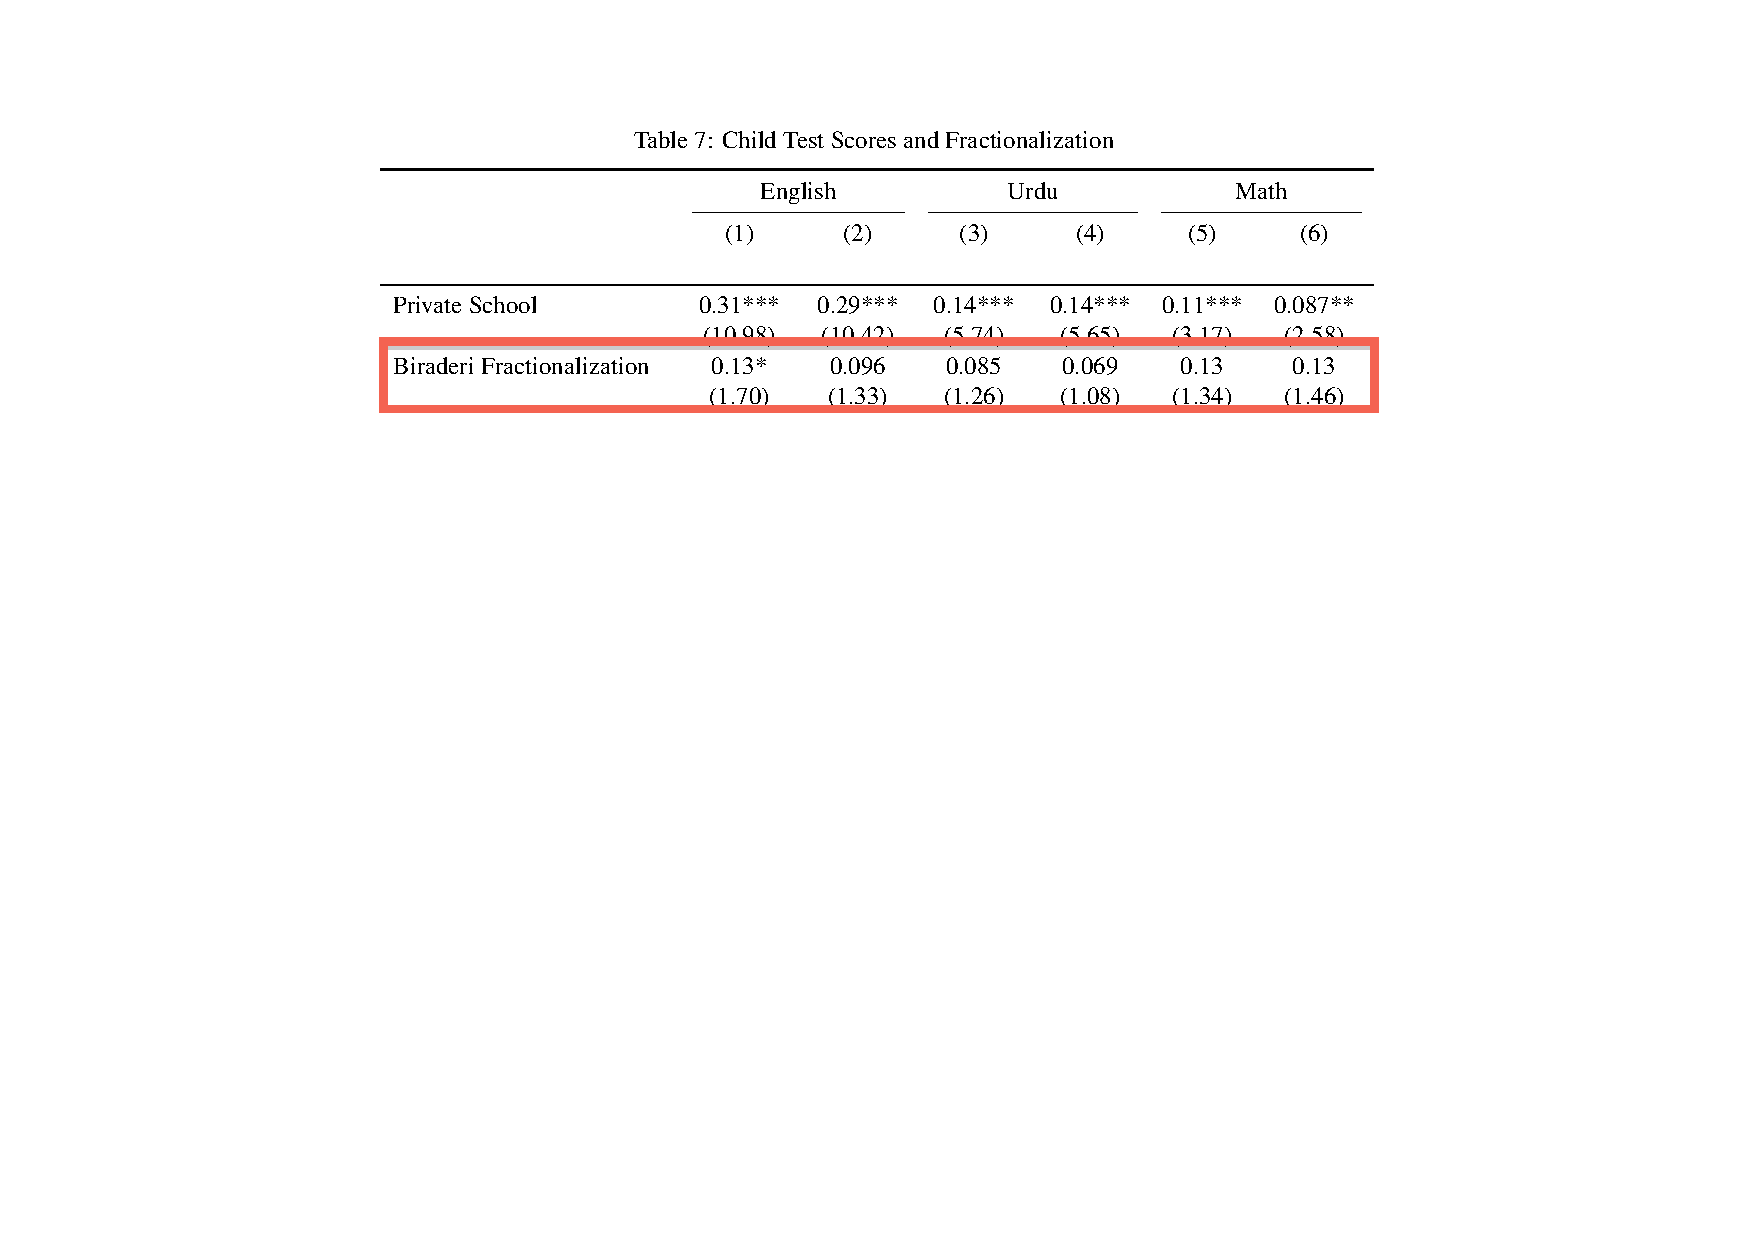
\includegraphics[scale=0.65]{tables/mean_preserving_box1.pdf}
		\end{center}
	\end{figure}
\end{frame}



\begin{frame}{}
	\begin{figure}[htb]
		\begin{center}
		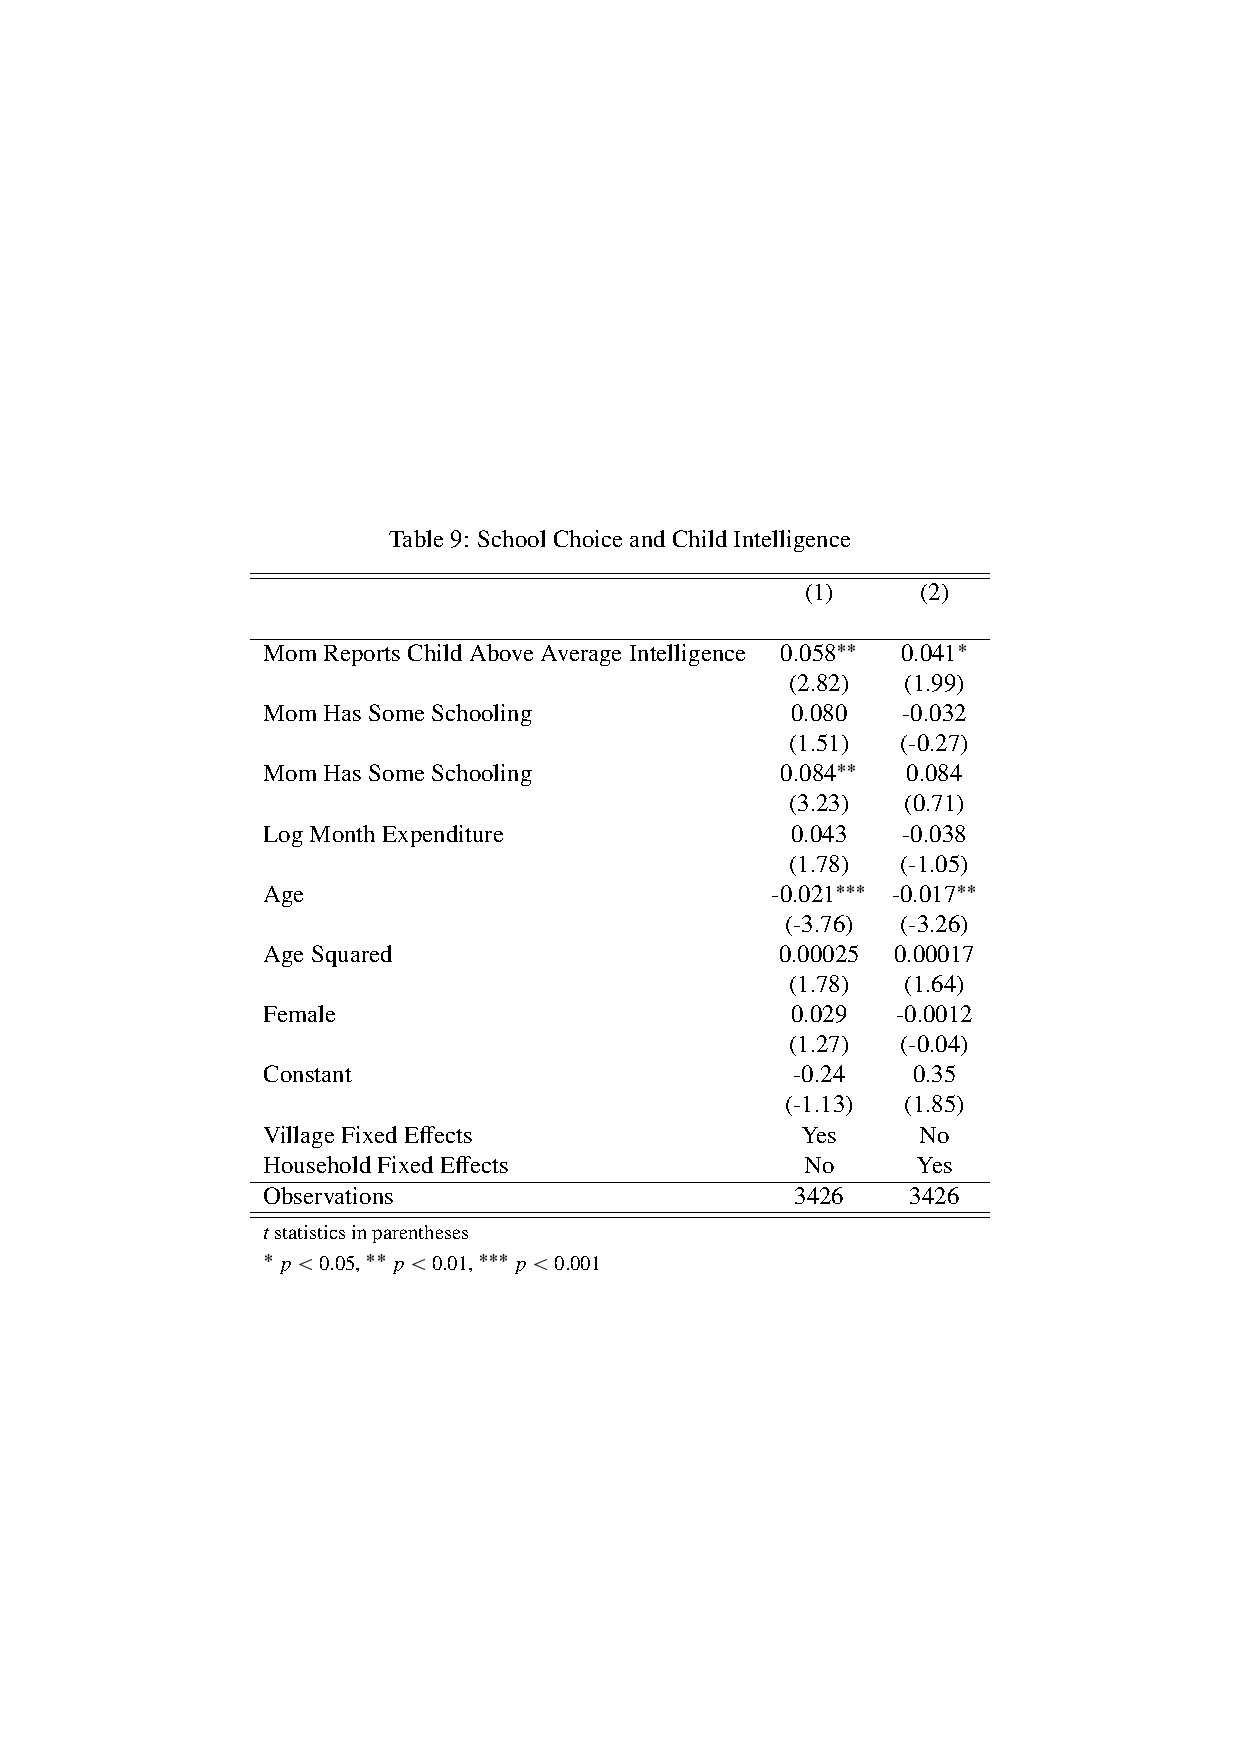
\includegraphics[scale=0.7]{tables/intelligence_type.pdf}
		\end{center}
	\end{figure}
\end{frame}

\begin{frame}{}
	\begin{figure}[htb]
		\begin{center}
		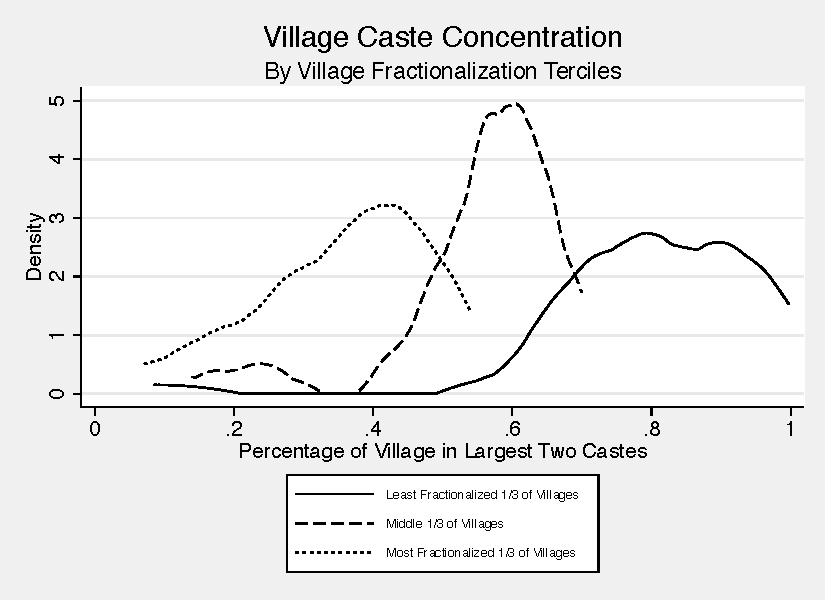
\includegraphics[scale=0.8]{graphs/village_toptwo.pdf}
		\end{center}
	\end{figure}
\end{frame}

\begin{frame}{}
	\begin{figure}[htb]
		\begin{center}
		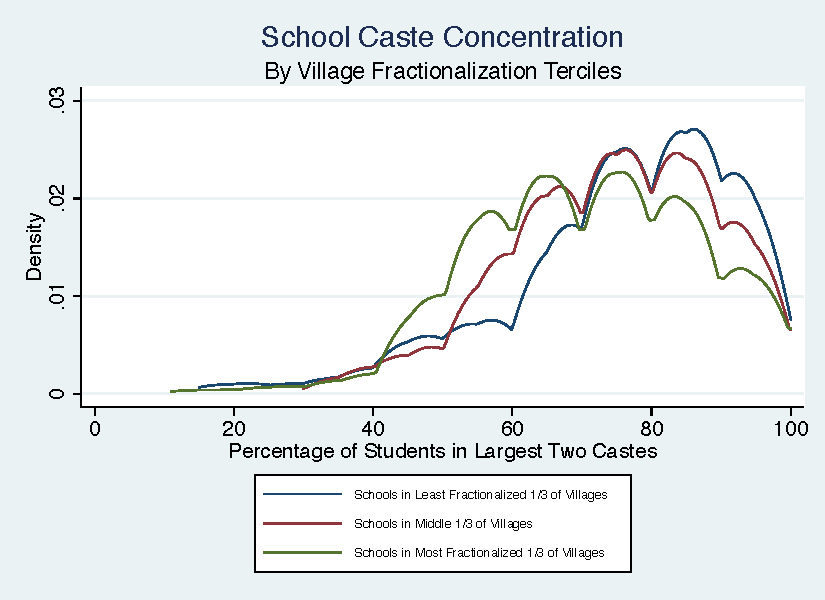
\includegraphics[scale=0.8]{graphs/school_toptwo.pdf}
		\end{center}
	\end{figure}
\end{frame}

\begin{frame}{}
	\begin{figure}[htb]
		\begin{center}		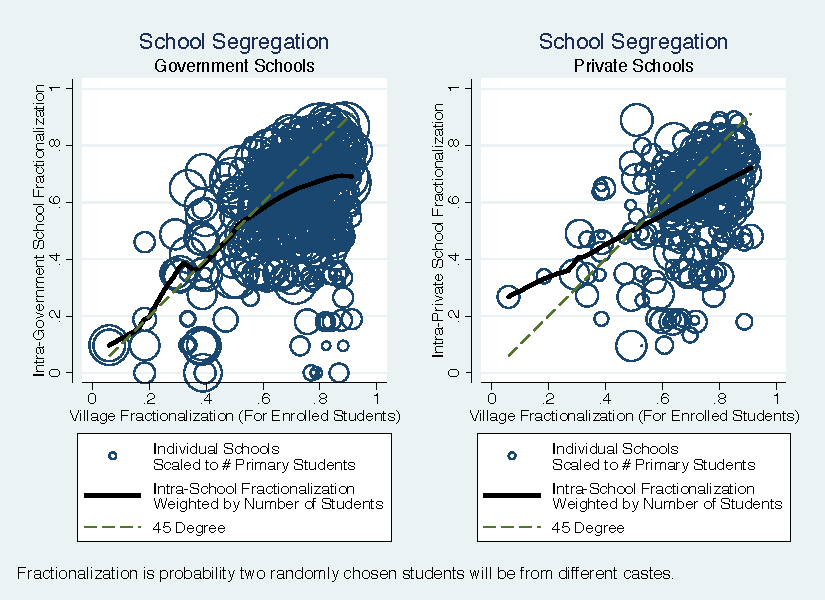
\includegraphics[scale=0.8]{graphs/intra_versus_intervillage_frac_combined.pdf}
		\end{center}
	\end{figure}
\end{frame}

\begin{frame}{}
	\begin{figure}[htb]
		\begin{center}
		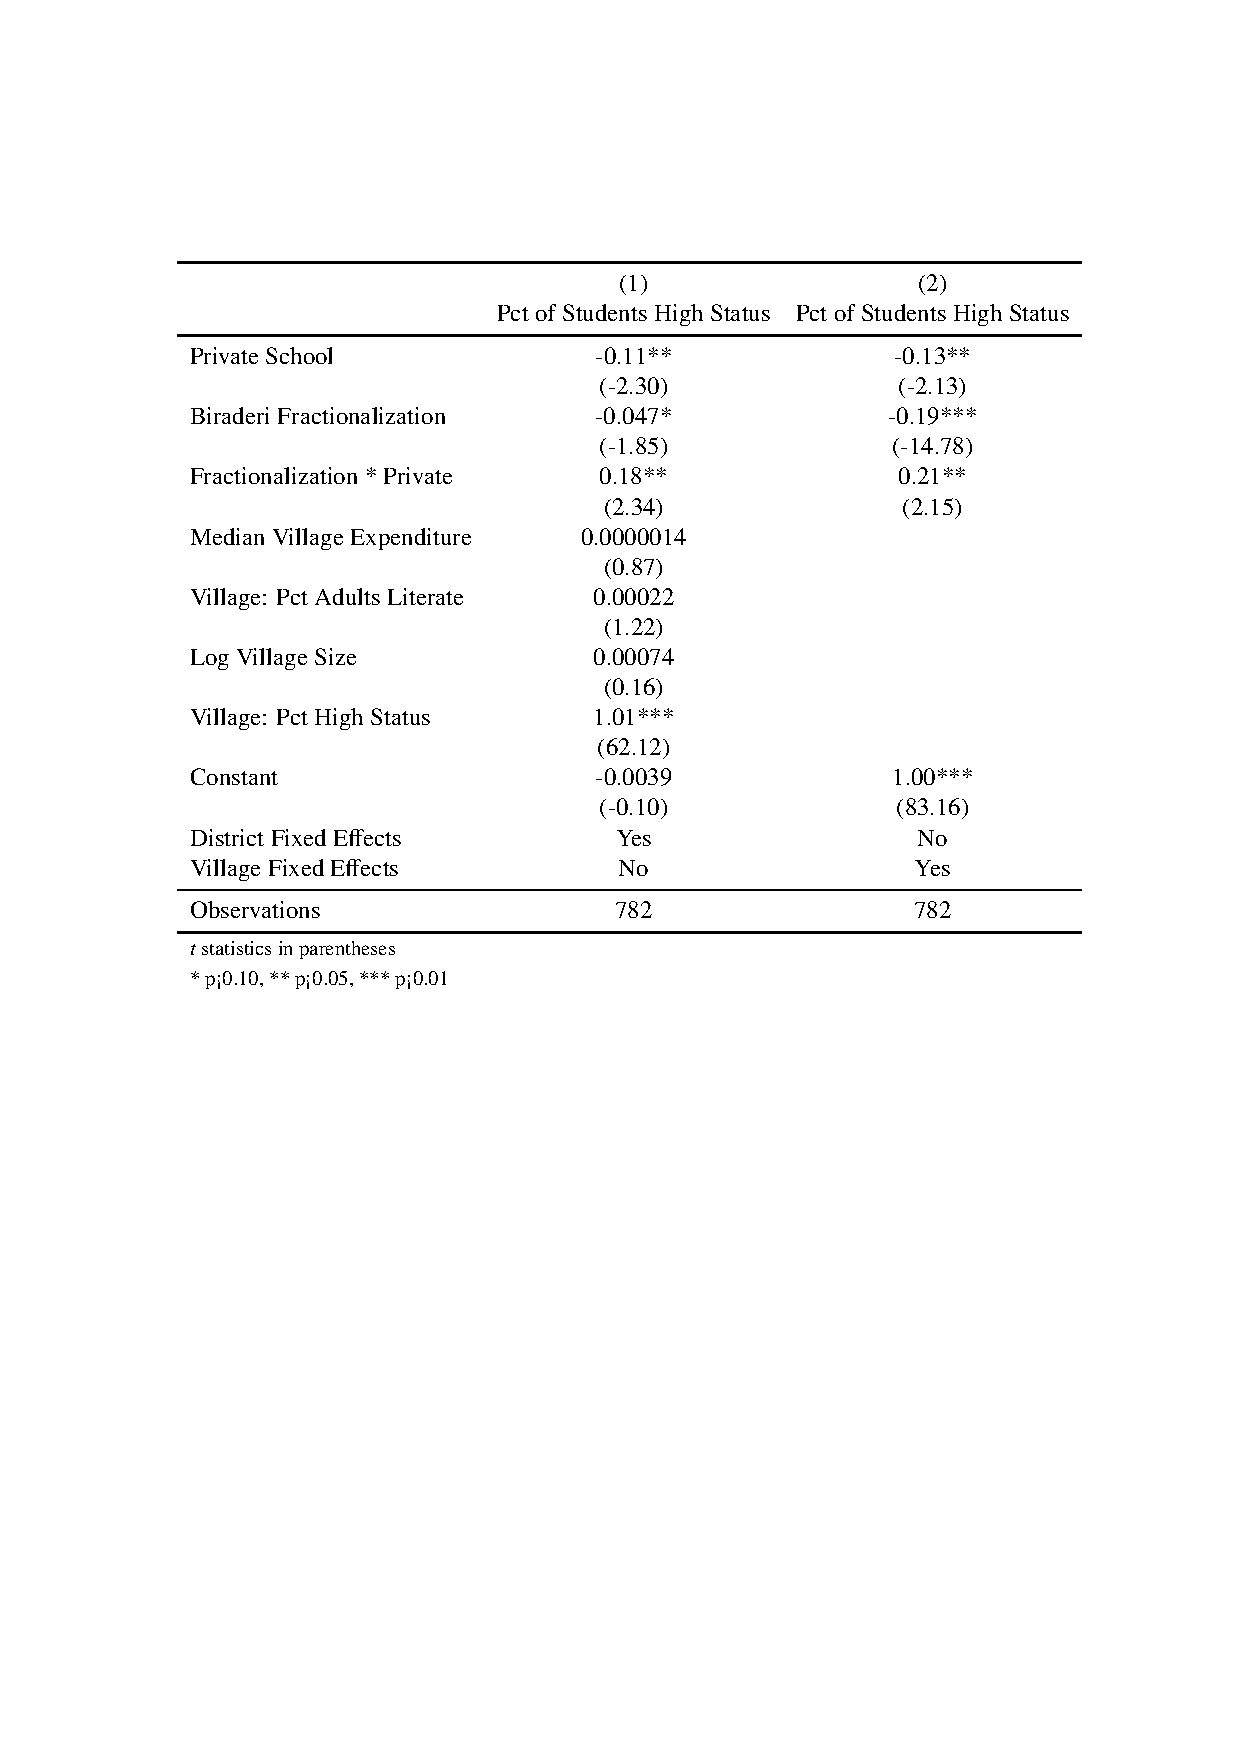
\includegraphics[scale=0.7]{tables/social_status_type.pdf}
		\end{center}
	\end{figure}
\end{frame}

\begin{frame}{}
	\begin{figure}[htb]
		\begin{center}
		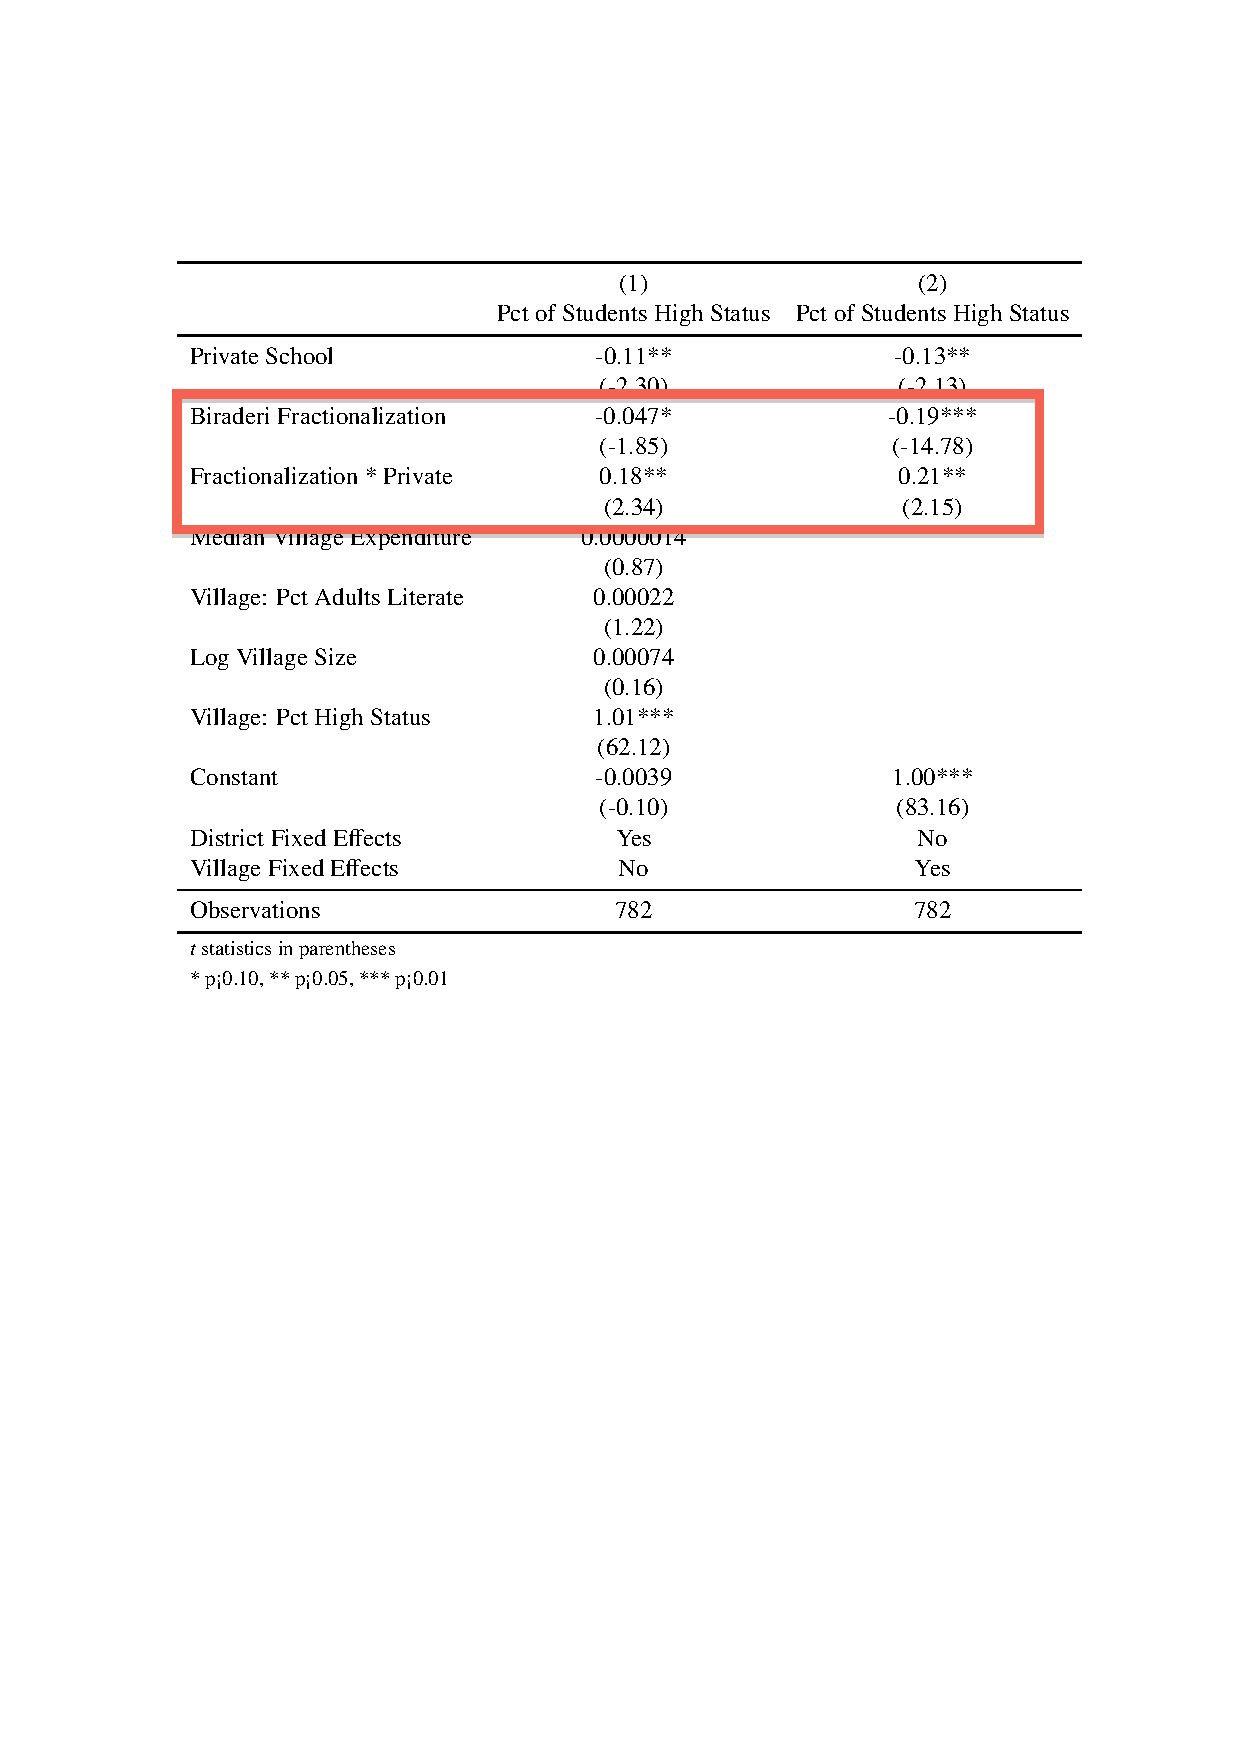
\includegraphics[scale=0.7]{tables/social_status_type_box1.pdf}
		\end{center}
	\end{figure}
\end{frame}


\begin{frame}{Fractionalization and Prices}
	\begin{figure}[htb]
		\begin{center}
		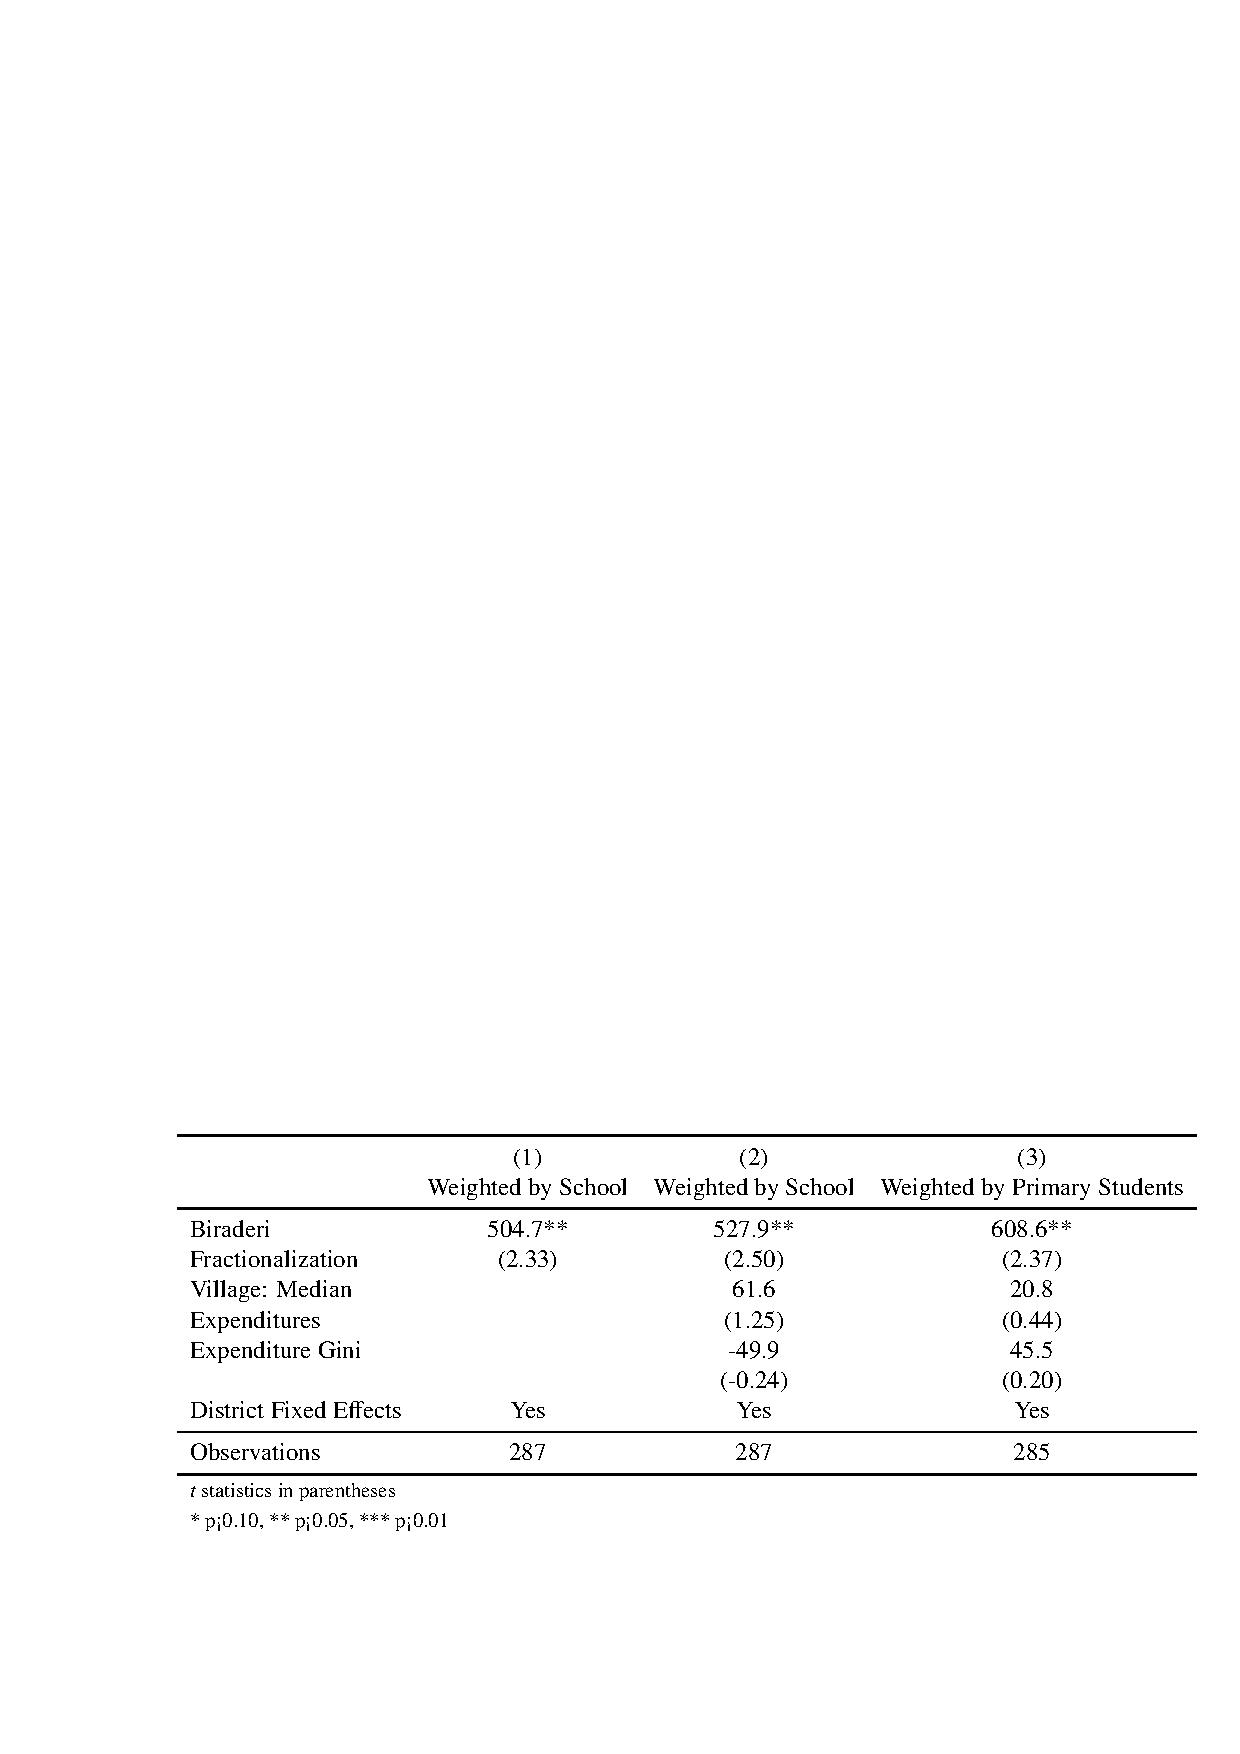
\includegraphics[scale=0.6]{tables/prices.pdf}
		\end{center}
	\end{figure}
\end{frame}

\begin{frame}{Inconsistencies}
\begin{figure}[htb]
	\begin{center}
	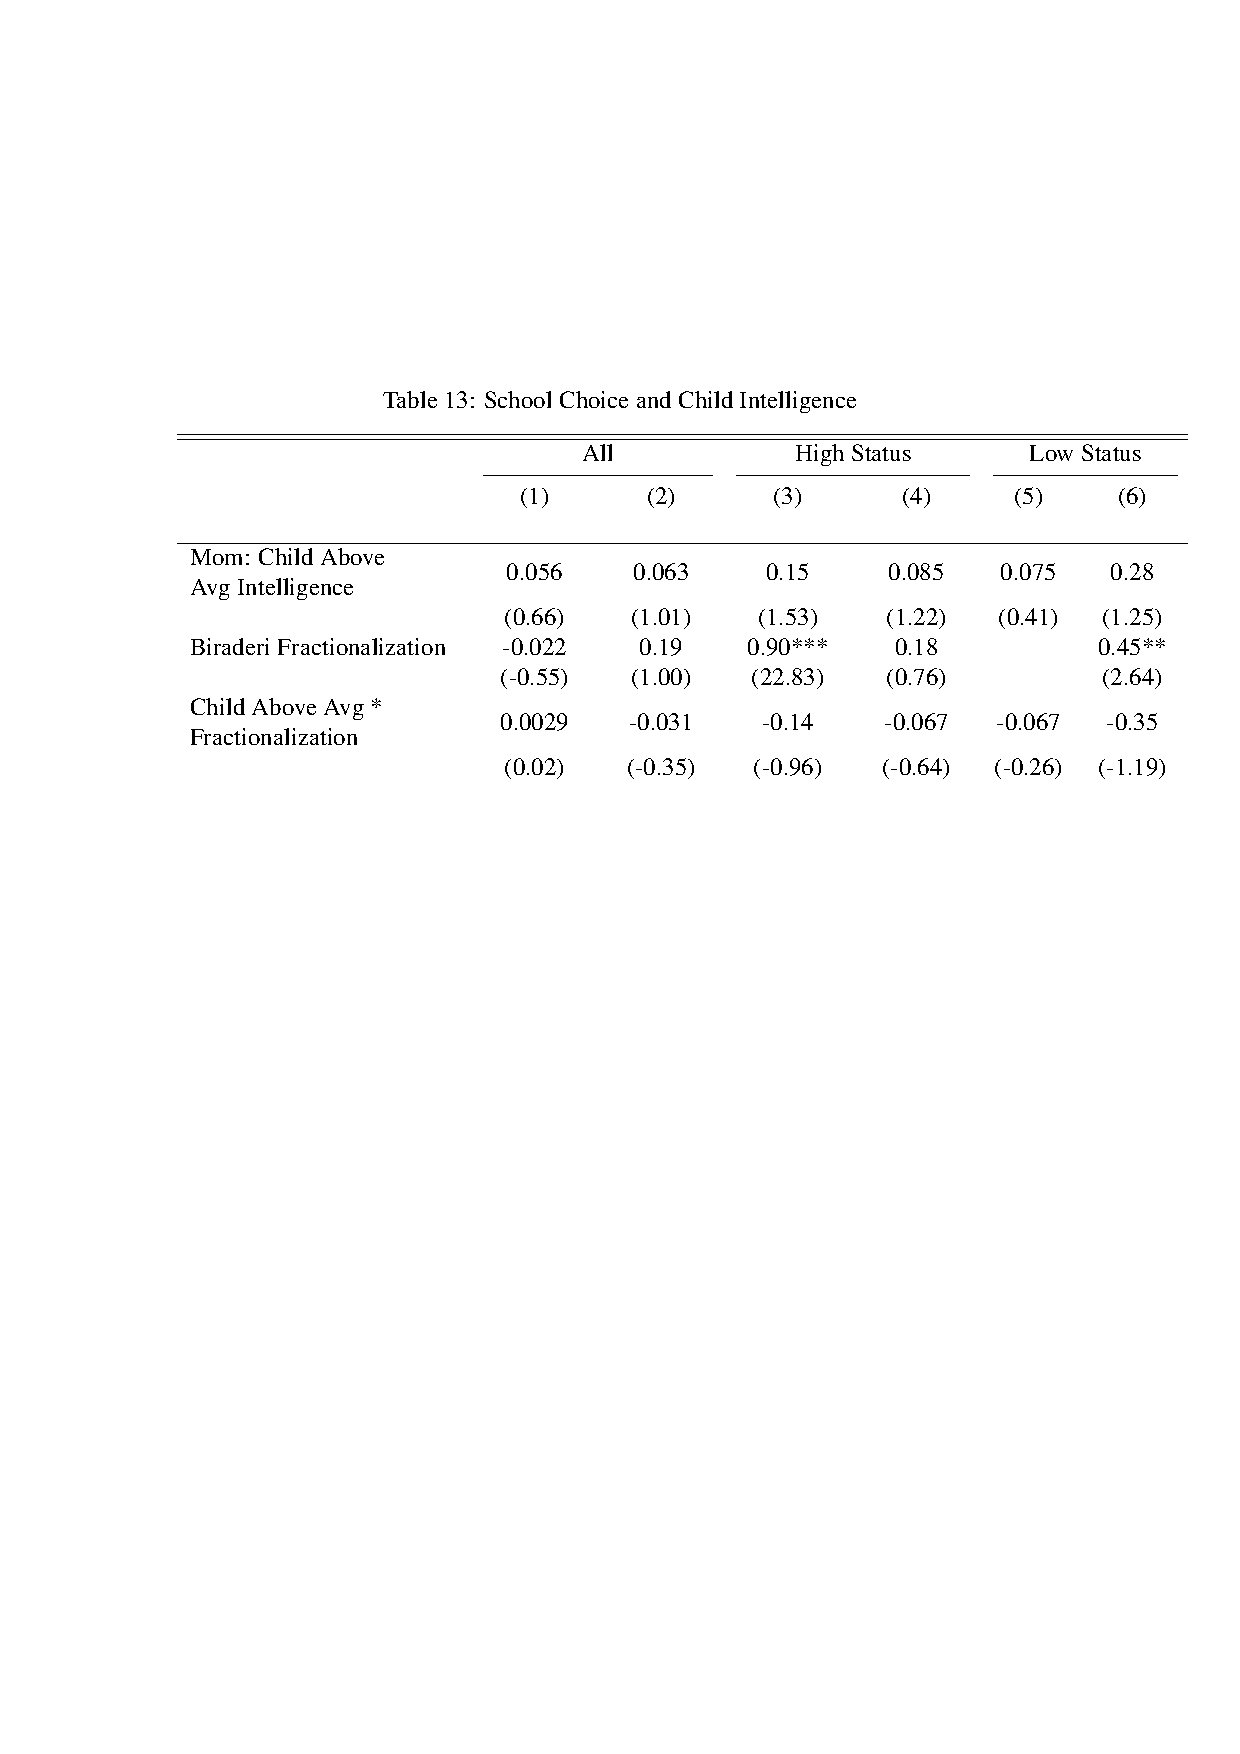
\includegraphics[scale=0.65]{tables/choice_interactions.pdf}
	\end{center}
\end{figure}

\end{frame}

\begin{frame}{Inconsistencies}
\begin{figure}[htb]
	\begin{center}
	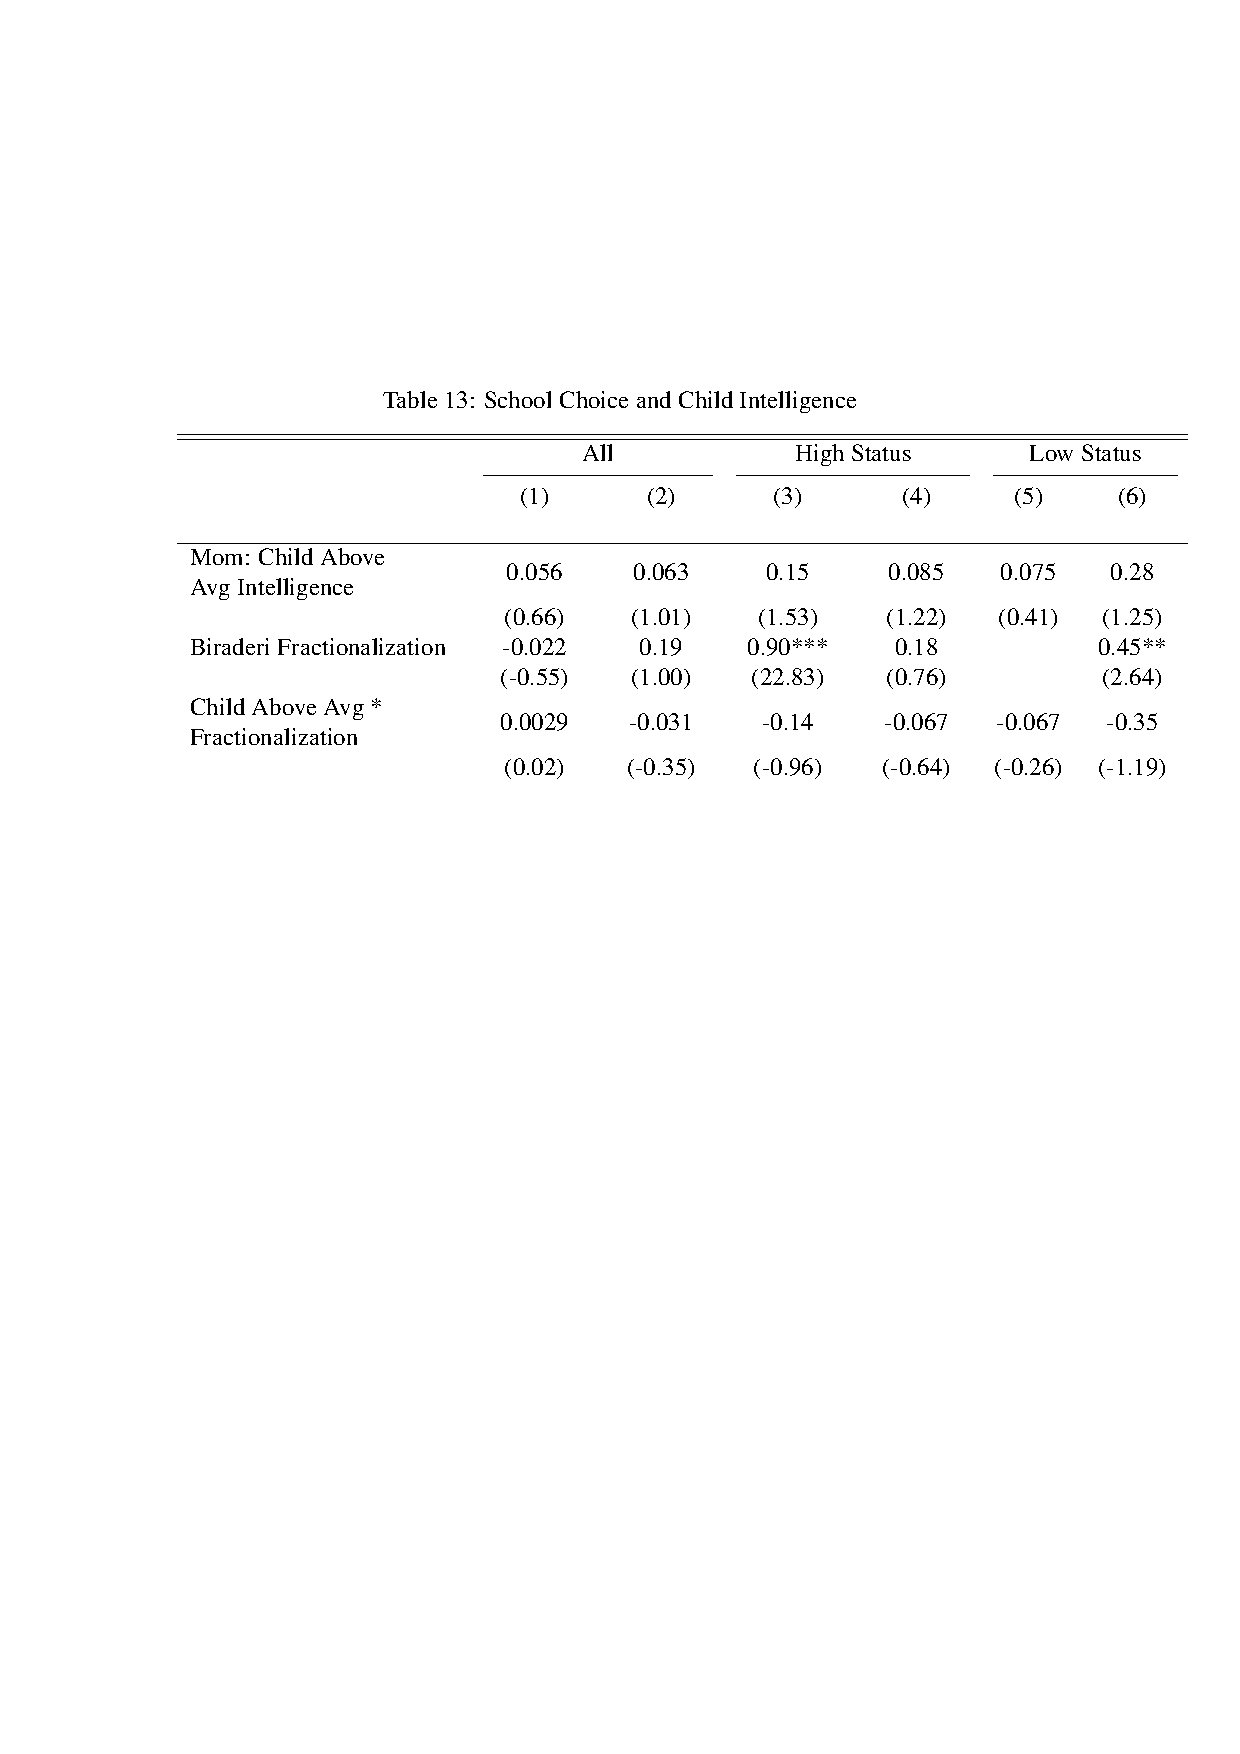
\includegraphics[scale=0.65]{tables/choice_interactions_box.pdf}
	\end{center}
\end{figure}

\end{frame}



\begin{frame}{Sorting Paradox}
Why pay more for the same education?
\pause
\begin{description}
	\item [Neighborhood Effects:] Students performance is affected by peers
	\pause
	\item [Networking:] About forming positive associations. 
	\begin{itemize}
		\item In homogenous villages, most important association is intelligence.
		\item In fractionalized villages, caste matters too. 
	\end{itemize}
\end{description}
\end{frame}


\section{Summary}\label{}
\begin{frame}{Outline}
	\tableofcontents[current]
\end{frame}



\begin{frame}{Conclusion}
Take-aways:
	\begin{enumerate}
		\item \emph{At least} 50\% of private school premium due to sorting.
		\pause
		\item Studying village characteristics can provide new insights into role of sorting.
	\end{enumerate}
\pause
Next Steps:
\begin{itemize}
	\item Develop more robust measures of social status.
	\item Test in India
\end{itemize}

\pause
Things I would like from you:
\begin{itemize}
	\item Alternative explanations for convergence?
	\item Alternative tests for this explanation?
\end{itemize}

\end{frame}
\end{document}